\documentclass[pdftex,10pt,a4paper]{report}

\usepackage[pdftex]{graphicx}

\newcommand{\HRule}{\rule{\linewidth}{0.5mm}}
\usepackage{apacite}
\usepackage{fullpage}
\setcounter{tocdepth}{3}
\setcounter{secnumdepth}{0}
\usepackage{indentfirst}
\usepackage{wrapfig}
\usepackage{lipsum}
\usepackage[procnames]{listings}
\usepackage{hyperref}
\usepackage{caption}
\usepackage{subcaption}
\usepackage[usenames,dvipsnames]{color}
\hypersetup{
    colorlinks,
    citecolor=black,
    filecolor=black,
    linkcolor=black,
    urlcolor=black
}
\renewcommand{\baselinestretch}{1.5}
\makeatletter
\def\@makechapterhead#1{%
  \vspace*{50\p@}%
  {\parindent \z@ \raggedright \normalfont
    \interlinepenalty\@M
    \Huge \bfseries #1\par\nobreak
    \vskip 40\p@
  }}
  \makeatother
 

\begin{document}
\definecolor{keywords}{RGB}{255,0,90}
\definecolor{comments}{RGB}{0,0,113}
\definecolor{red}{RGB}{160,0,0}
\definecolor{green}{RGB}{0,150,0}
 \definecolor{string}{rgb}{0.7,0.0,0.0}
 \definecolor{gray}{RGB}{47,47,47}
\lstset{language=Python, 
        basicstyle=\ttfamily\small, 
        keywordstyle=\bf\color{keywords},
        commentstyle=\color{comments},
	otherkeywords={self},
        stringstyle=\color{red},
        showstringspaces=false,
        identifierstyle=\color{gray}}

\begin{titlepage}
\begin{center}

% Upper part of the page. The '~' is needed because \\
% only works if a paragraph has started.

\includegraphics[width=0.25\textwidth]{img/group/logo.png}~\\[1cm]

\textsc{\LARGE University of Toronto}\\[0.7cm]

\textsc{\Large CSCD01 Phase 1 Report}\\
\textsc{\large Team: Infinity}\\[0.5cm]

% Title
\HRule \\[0.4cm]
{ \huge \bfseries Reverse Engineering \\[0.4cm] }

\HRule \\[1.5cm]

% Author and supervisor
\begin{minipage}{0.4\textwidth}
\begin{flushleft} \large
Andrew \textsc{Berneshawi}\\
Nicholas \textsc{Dujay}\\
Pirave \textsc{Eahalaivan}\\
Josh \textsc{Hillen}\\
Yunqin \textsc{Huang}\\
Ho-Cheung \textsc{Lai}\\
Wei \textsc{Li}\\
Choi \textsc{Tak}\\
\end{flushleft}
\end{minipage}
\begin{minipage}{0.4\textwidth}
\begin{flushright} \large
{\tt bernesha} 998425388\\
{\tt dujaynic} 999194900\\
{\tt eahalaiv} 998152136\\
{\tt hillenjo} 999143911\\
{\tt huangy11} 996445217\\
{\tt laihoche} 999035020\\
{\tt liwei18} 999232753\\
{\tt choitak} 997905566\\
\end{flushright}
\end{minipage}

\vfill

% Bottom of the page
{\large \today}
\end{center}
\end{titlepage}

\begin{abstract}
The objective of this report is to reverse engineer a set of models from the {\tt matplotlib} source code to explain its design. The goal is to use UML to highlight the structure and behaviour of the code. The report strategically determines which aspects of the design to model, how much to abstract away from the code base, and which parts of UML to use. The models are designed to explain the most interesting and important aspects of the design.
\end{abstract}

\tableofcontents
\listoffigures

%xxxxxxxxxxxxxxxxxxxxxxxxxxxxxxxxxxxxxxxxxxxxxxxxxxxxxxxxxxx
%xxxxxxxxxxxxxxxxxxxxxxxxxxxxxxxxxxxxxxxxxxxxxxxxxxxxxxxxxxx
% BEGIN DOCUMENT
%xxxxxxxxxxxxxxxxxxxxxxxxxxxxxxxxxxxxxxxxxxxxxxxxxxxxxxxxxxx
%xxxxxxxxxxxxxxxxxxxxxxxxxxxxxxxxxxxxxxxxxxxxxxxxxxxxxxxxxxx
\chapter{Introduction}

\section{Team}

  \begin{center}
    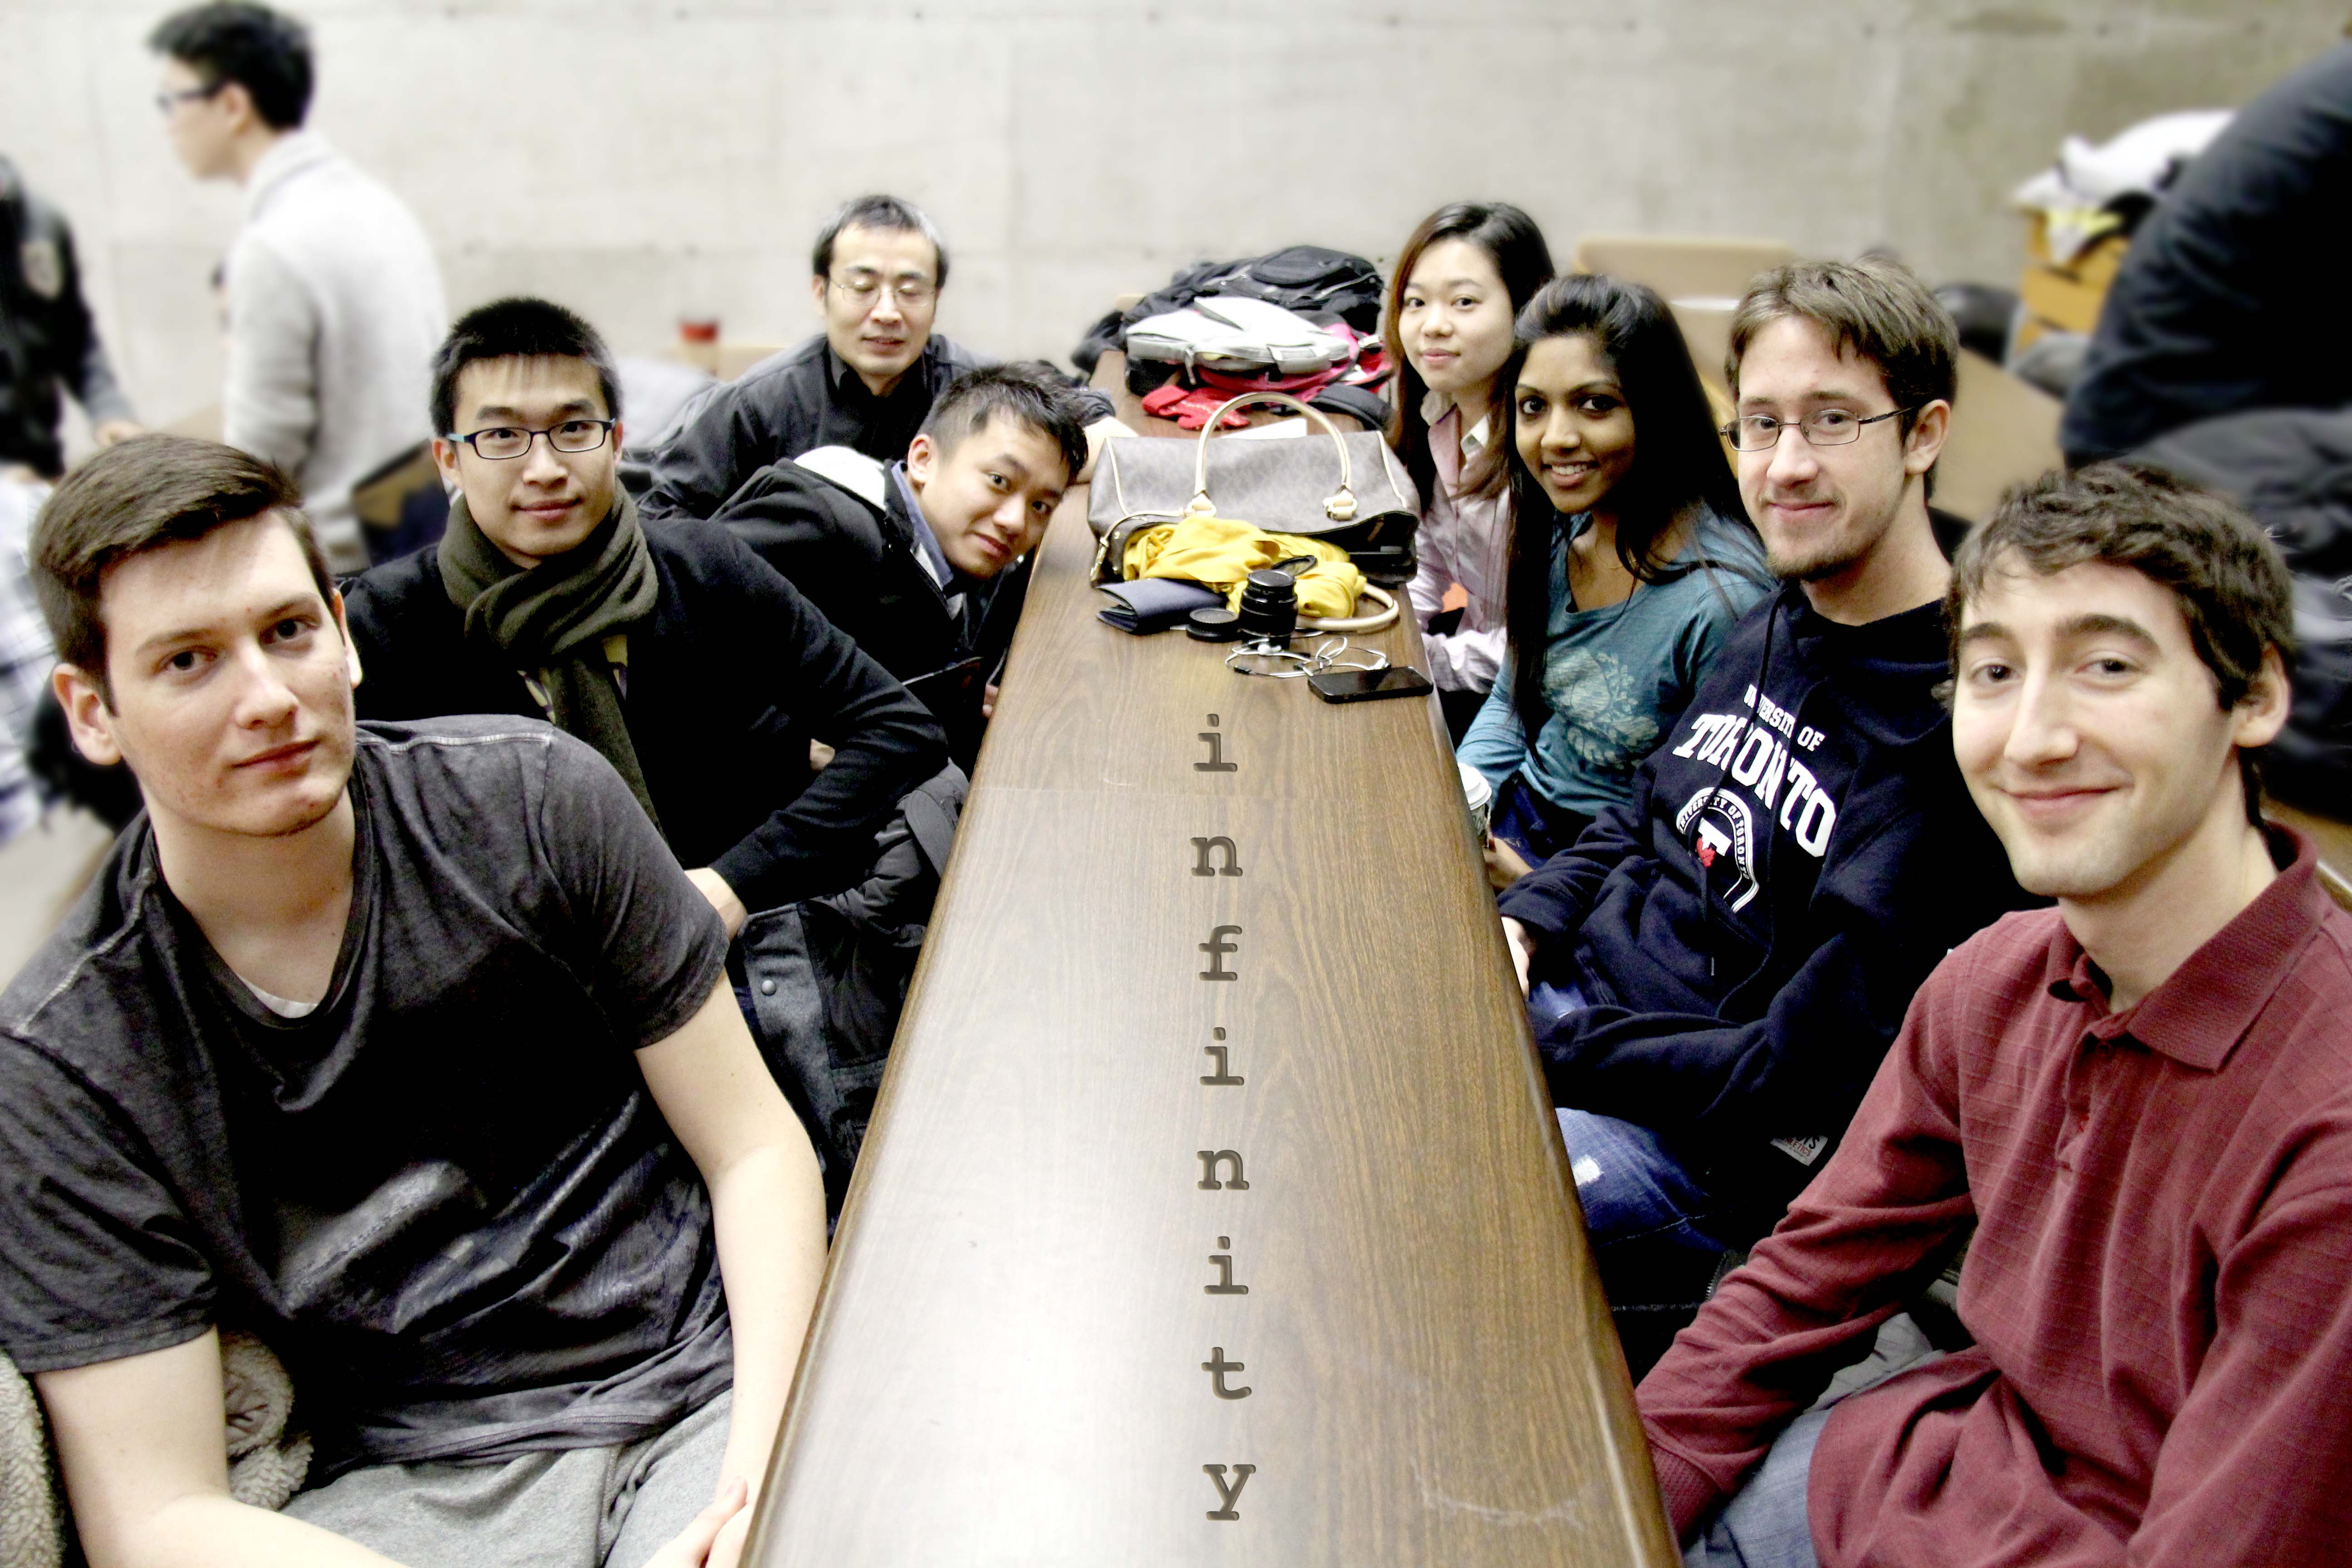
\includegraphics[width=1\textwidth]{img/group/group}
  \end{center}
We are team $\infty$.
\newpage
\section{Members}
\begin{wrapfigure}{l}{0.25\textwidth}
  \vspace{-20pt}
  \begin{center}
    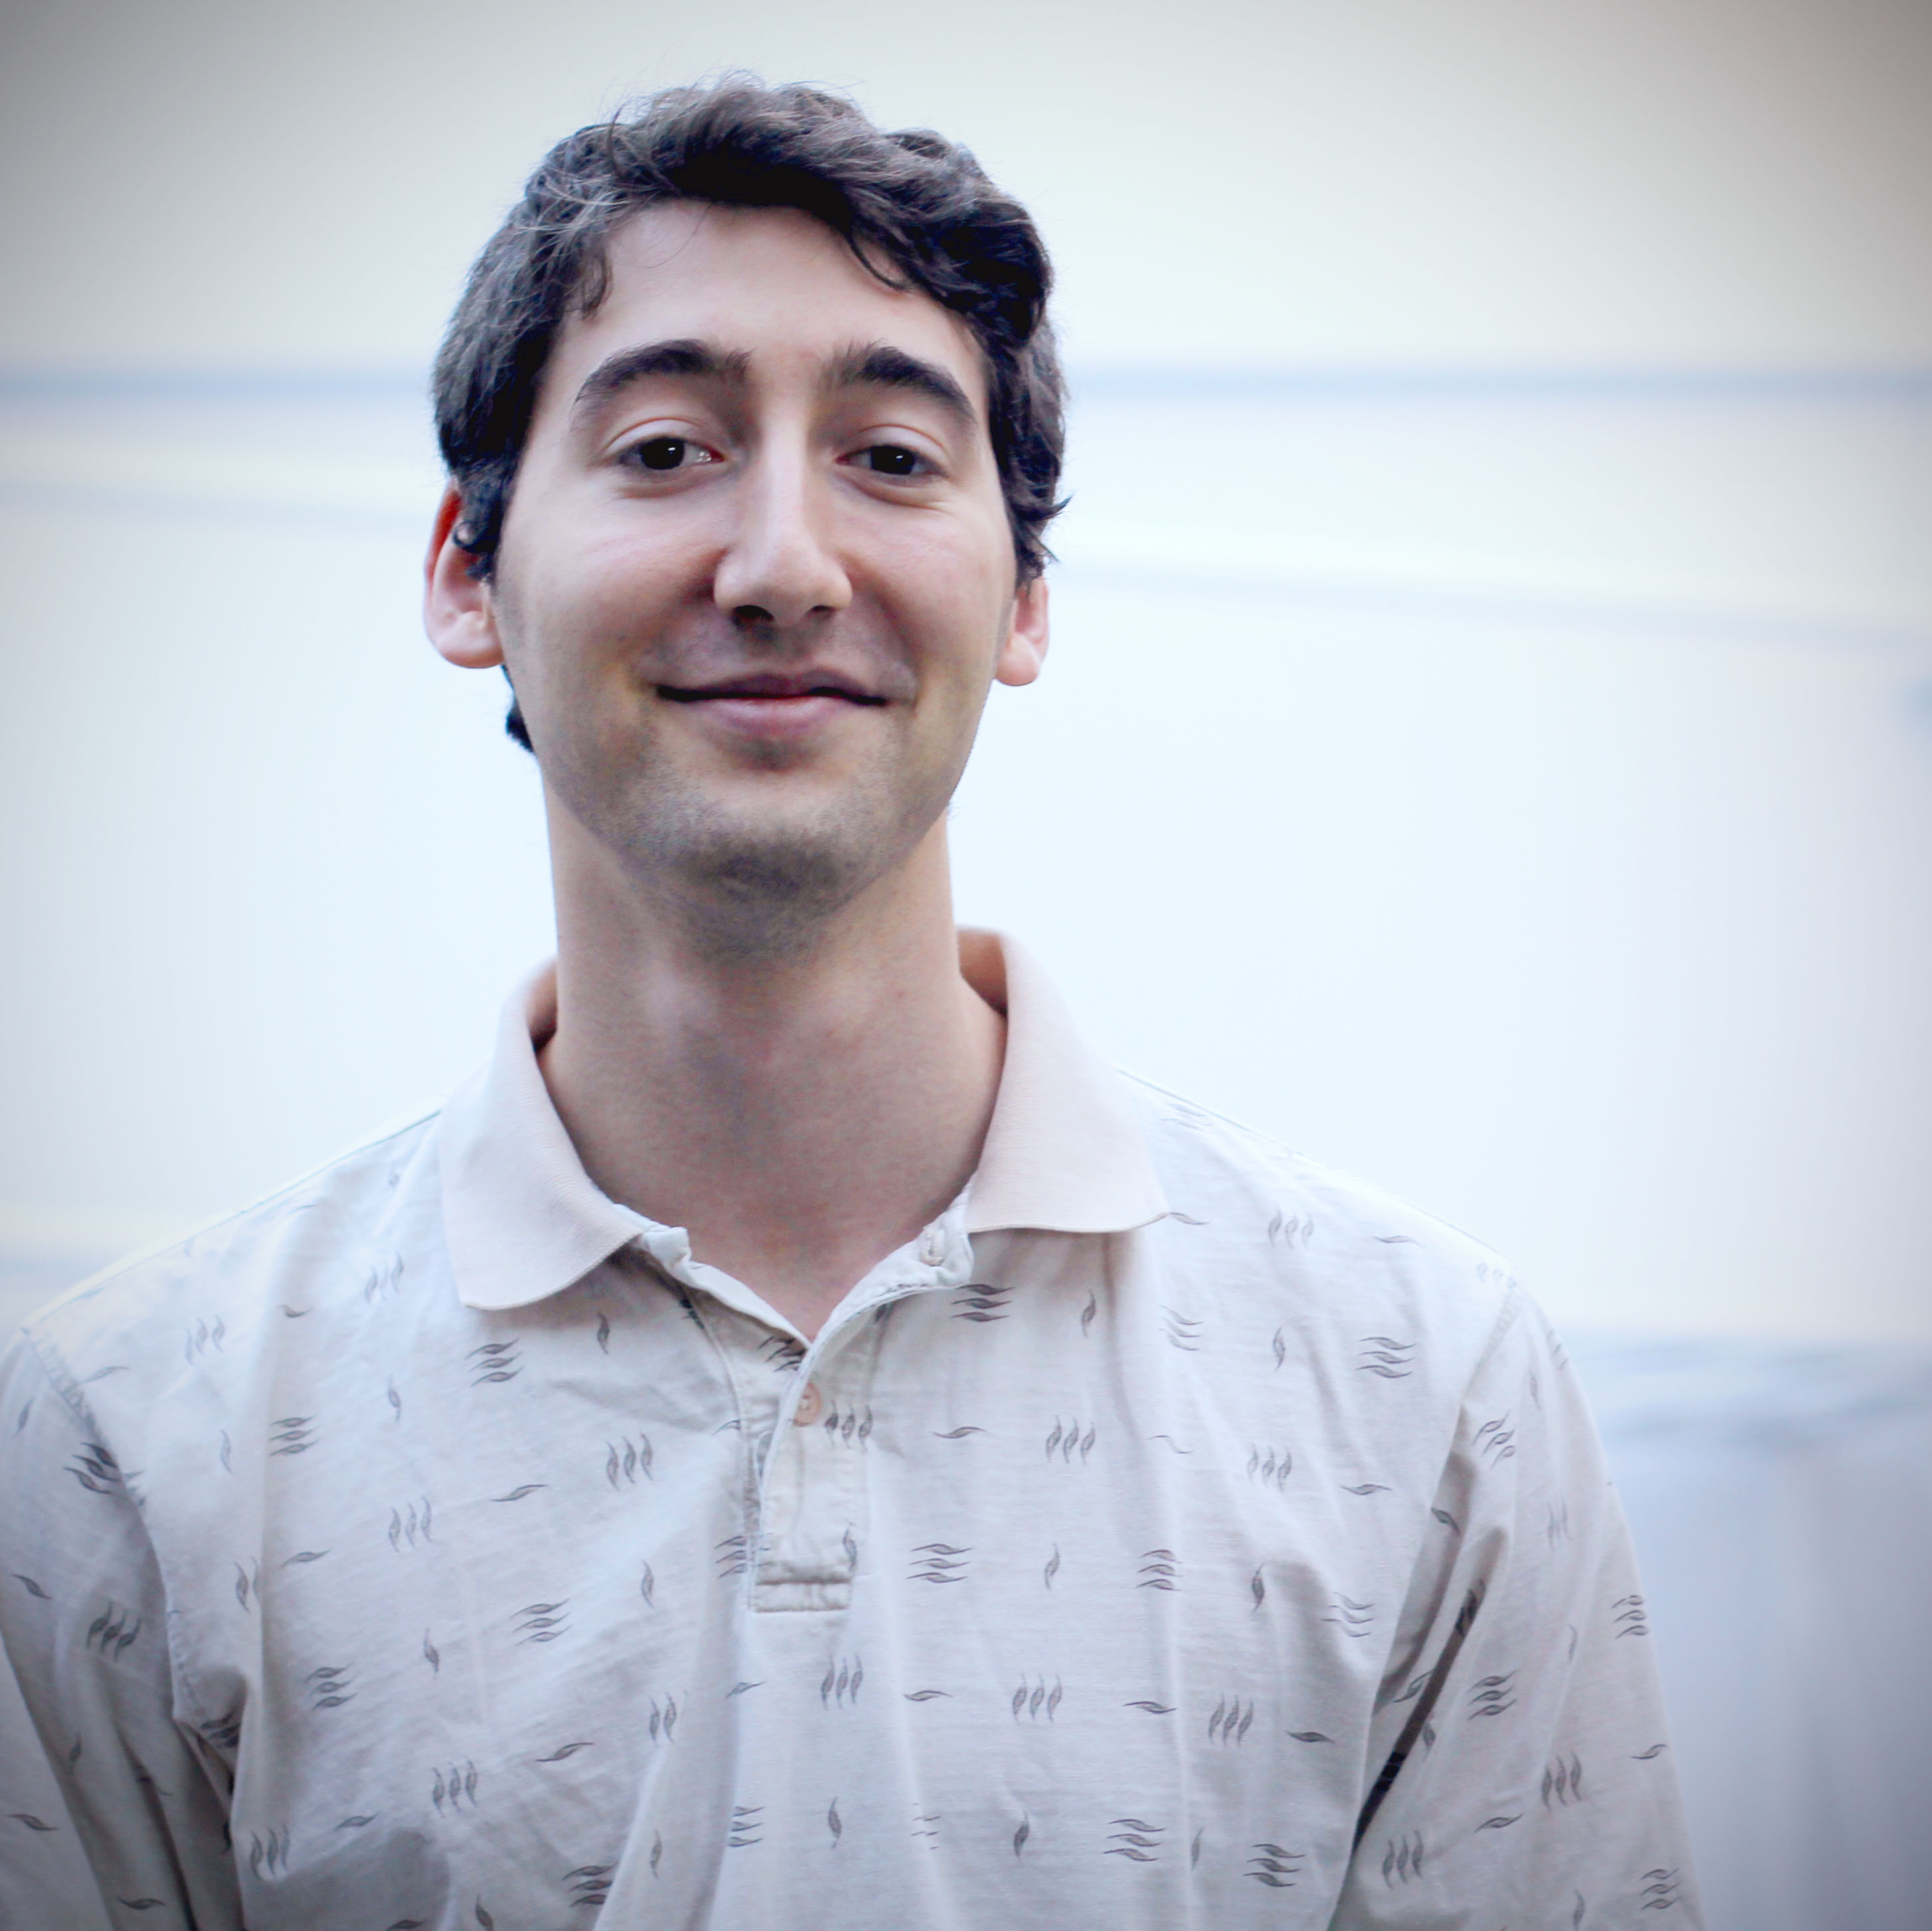
\includegraphics[width=0.25\textwidth]{img/group/andrew}
  \end{center}
  \vspace{-20pt}
\end{wrapfigure}
 Andrew Berneshawi is currently in the 3rd year of his Computer Science Specialist program in the Software Engineering stream. Thanks to his involvement in the co-op program he already has over a year of industry experience in web development. In his first internship at UTSC's IITS department he worked with PHP, followed by Java at IBM, and Java again in his latest job at Amazon; where he also gained experience with agile development. Now that he is back in class he looks forward to strengthening other parts of his software development knowledge. Not just passionate about software, Andrew also enjoys staying up to date on the latest computer hardware, and has built a few computers for his friends and himself. Outside of computer science he is interested in the sciences in general, and although the course load has been prohibitive regarding taking any challenging physics or chemistry courses, he did manage to squeeze in some psychology courses which he found very interesting. He is looking forward to using his experience from previous courses and internships to contribute to the project. \\


\begin{wrapfigure}{l}{0.25\textwidth}
  \vspace{-20pt}
  \begin{center}
    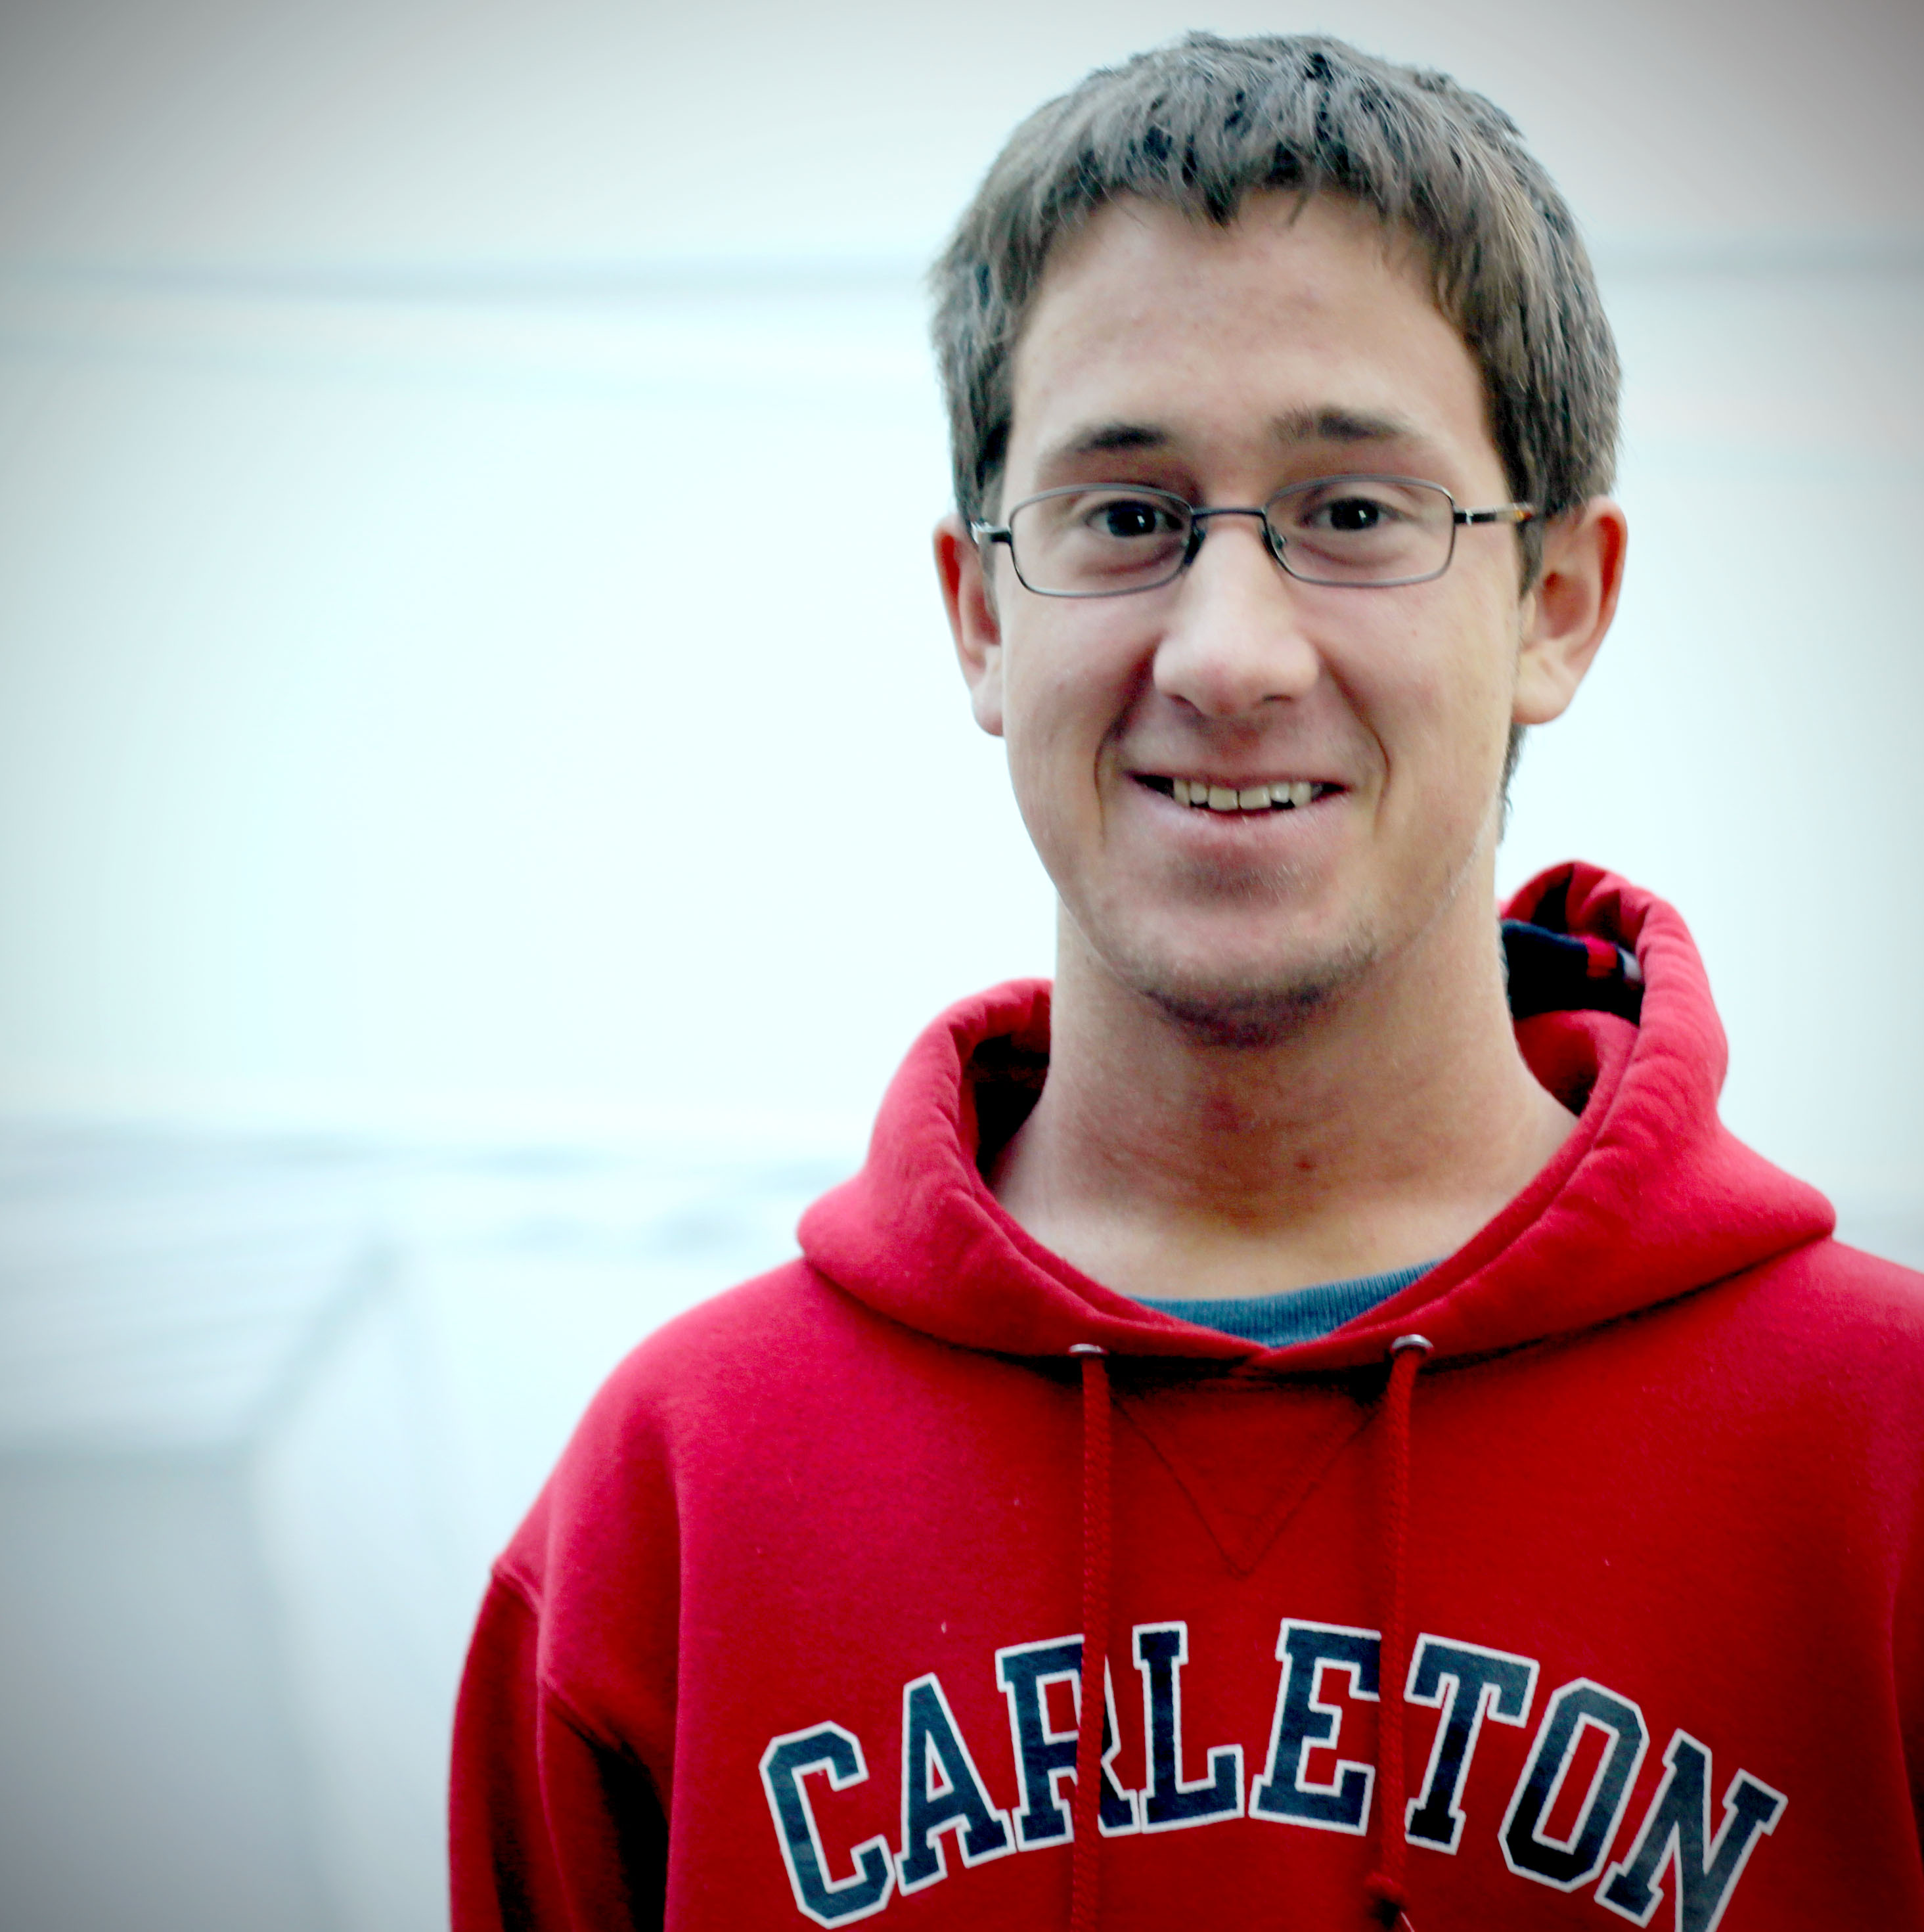
\includegraphics[width=0.25\textwidth]{img/group/nick}
  \end{center}
  \vspace{-20pt}
\end{wrapfigure}
Nicholas Dujay is a 3rd year undergraduate computer science student at the University of Toronto Scarborough Campus. He transferred from Carleton University, where he was studying to become an electrical engineer, but he decided to pursue his passion in computers and study at the University of Toronto. He is interested in learning agile, extreme programming and the software development process so he can have an idea of how software development happens in a real business setting. He is hoping to enter the video game industry after graduation, so this class will help him have an idea of how to work in a team. He spent a couple months developing a game during the summer of 2013, but had to stop development because of school. He has travelled to many places in North America, including Montreal, Moncton, New York, and Canc?n. In his spare time, he enjoys watching television shows such as Breaking Bad.\\


\begin{wrapfigure}{l}{0.25\textwidth}
  \vspace{-20pt}
  \begin{center}
    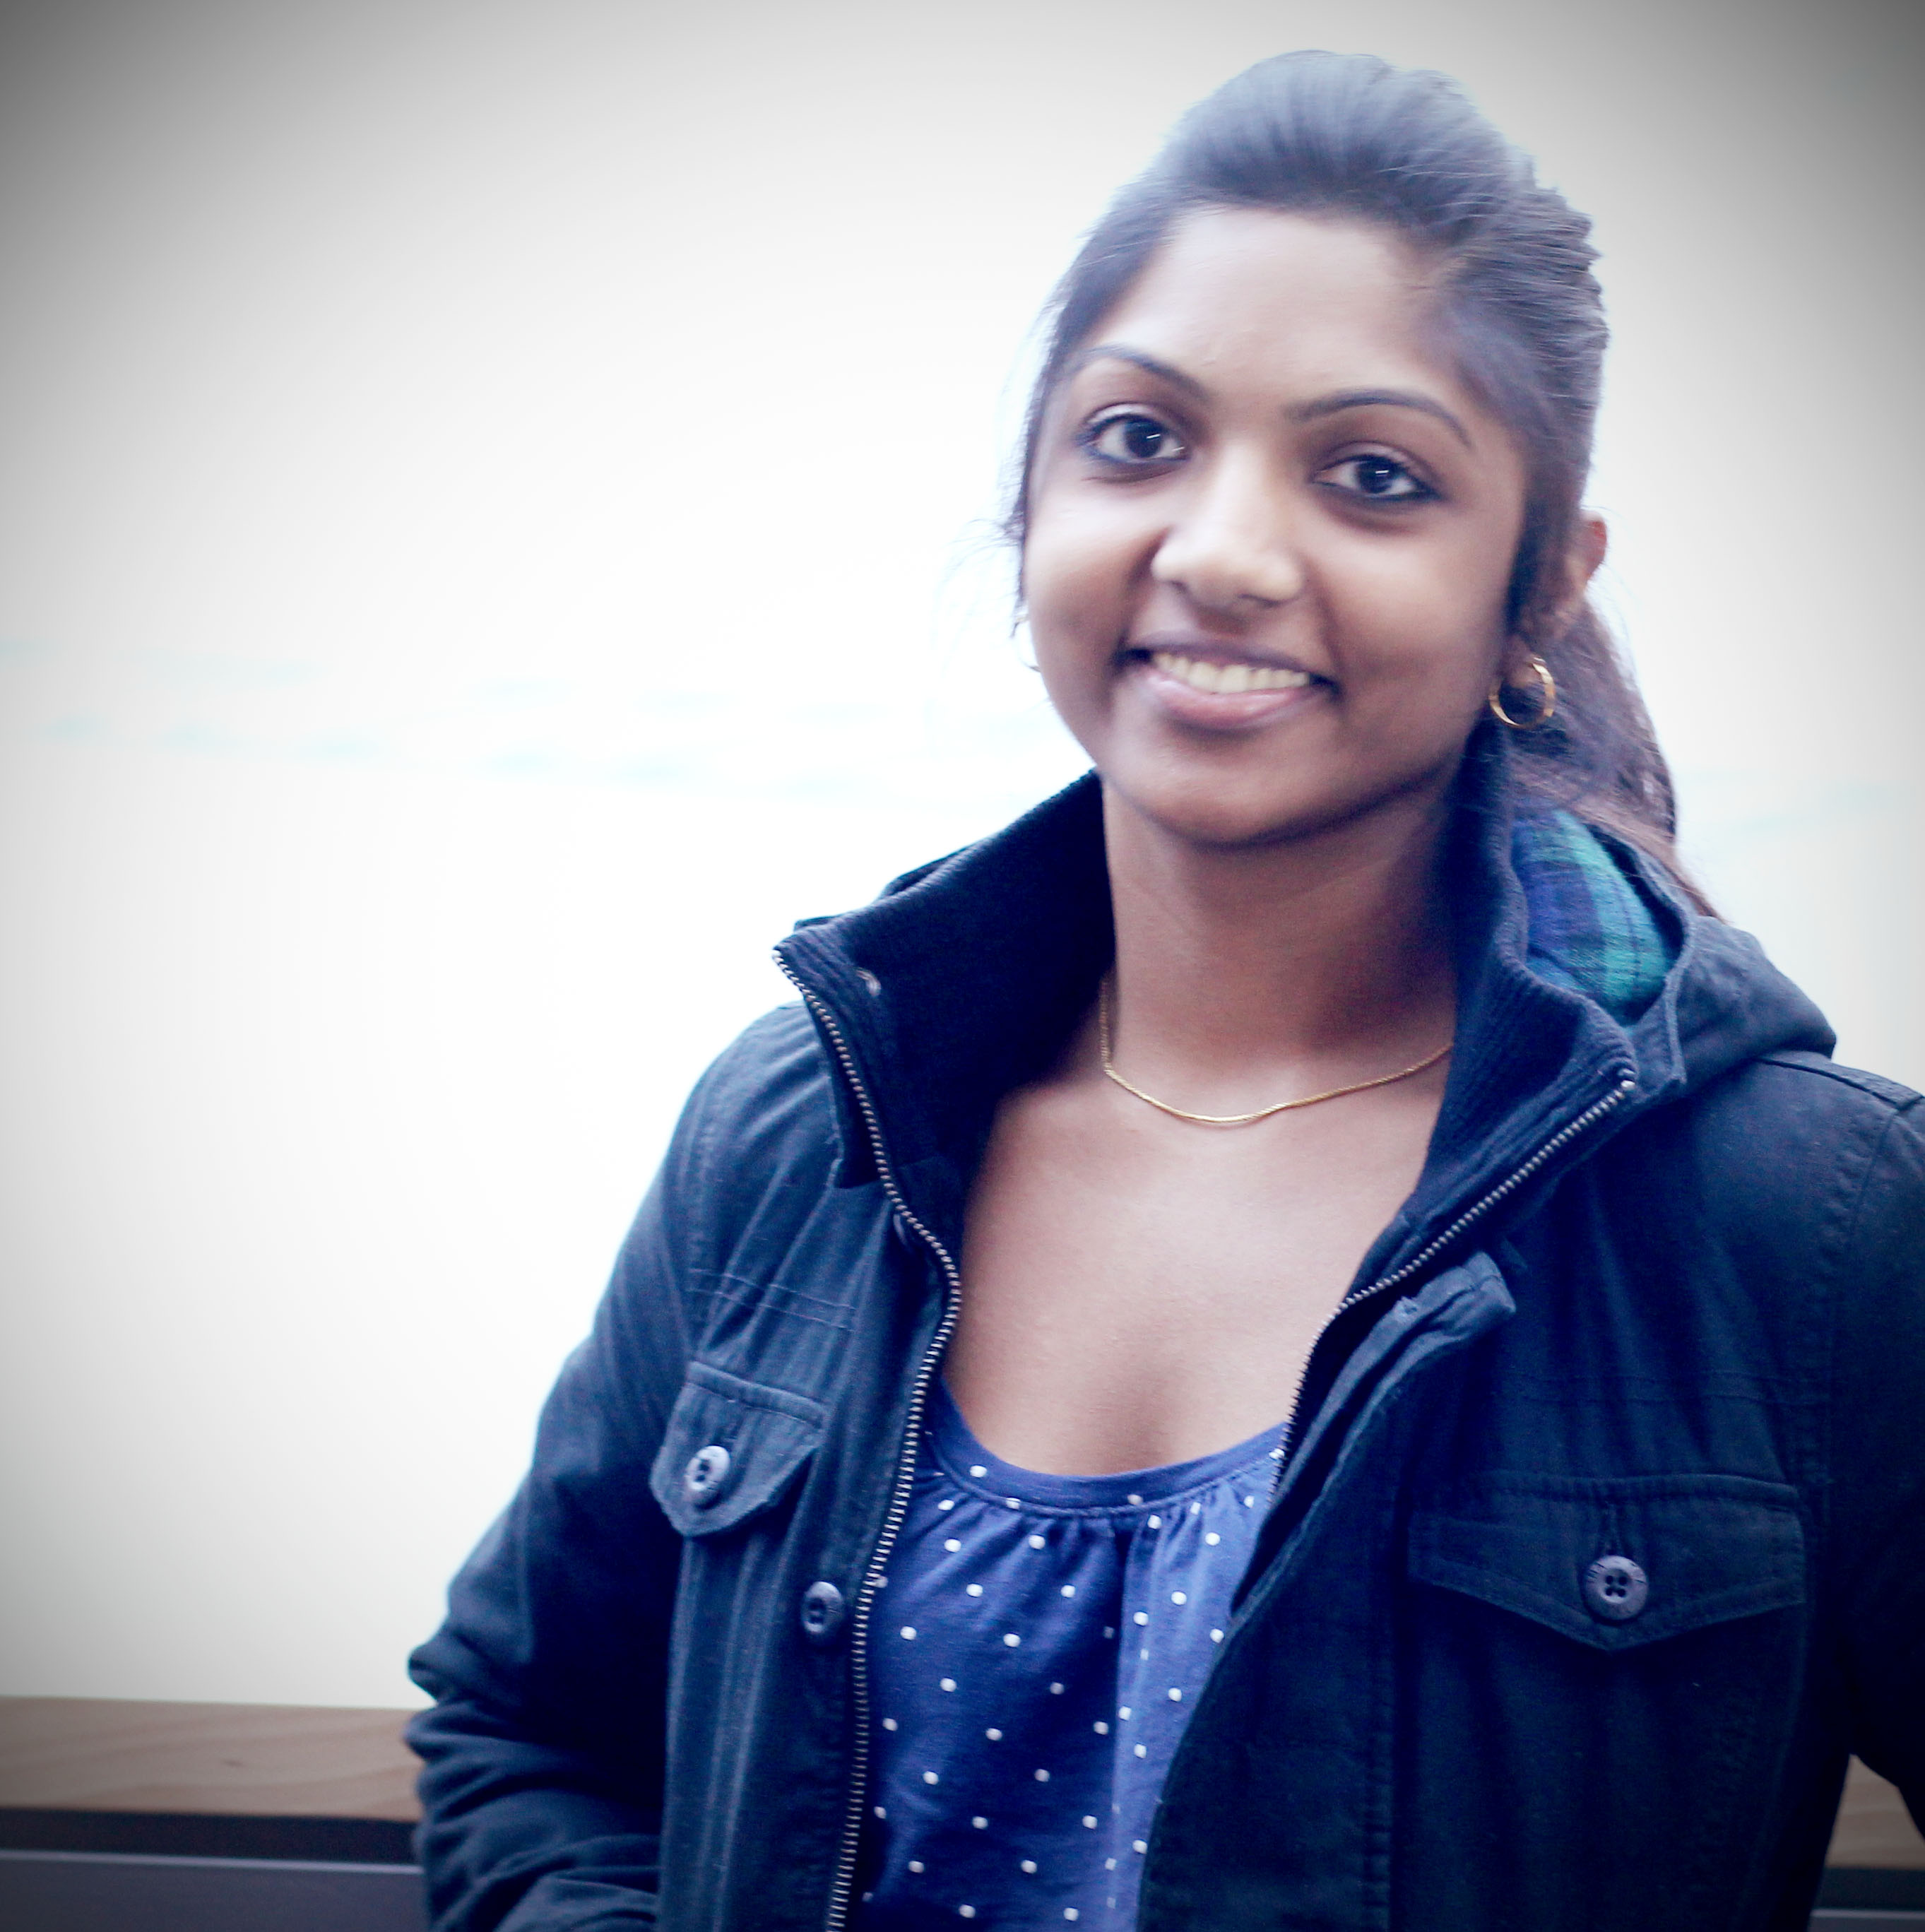
\includegraphics[width=0.25\textwidth]{img/group/pi}
  \end{center}
  \vspace{-20pt}
  \end{wrapfigure}
Pirave Eahalaivan is a 4th year student at the University of Toronto, specializing in computer science and minoring in psychology. As a part of the co-op program she has worked as a programmer analyst at Scotiabank and Ontario Teachers'Pension Plan. Her work experience has allowed her to explore web development via ASP.NET. These experiences have also enabled her to work in an agile developing environment. As the web associate for UofT's Co-op Student Association, she is responsible for designing, updating, and maintaining the club's website, using webpress. Having taken Programming on the Web (CSC309) and Databases (CSCC43), she has experience working front and back end with javascript, PHP, and MySQL. She would like to expand her horizons in web developing as well as graphic designing. She hopes to pursue a graduate degree in applied computing before she begins her career. Some of Pirave's hobbies include photography, reading and fitness.\\


\begin{wrapfigure}{l}{0.25\textwidth}
  \vspace{-20pt}
  \begin{center}
    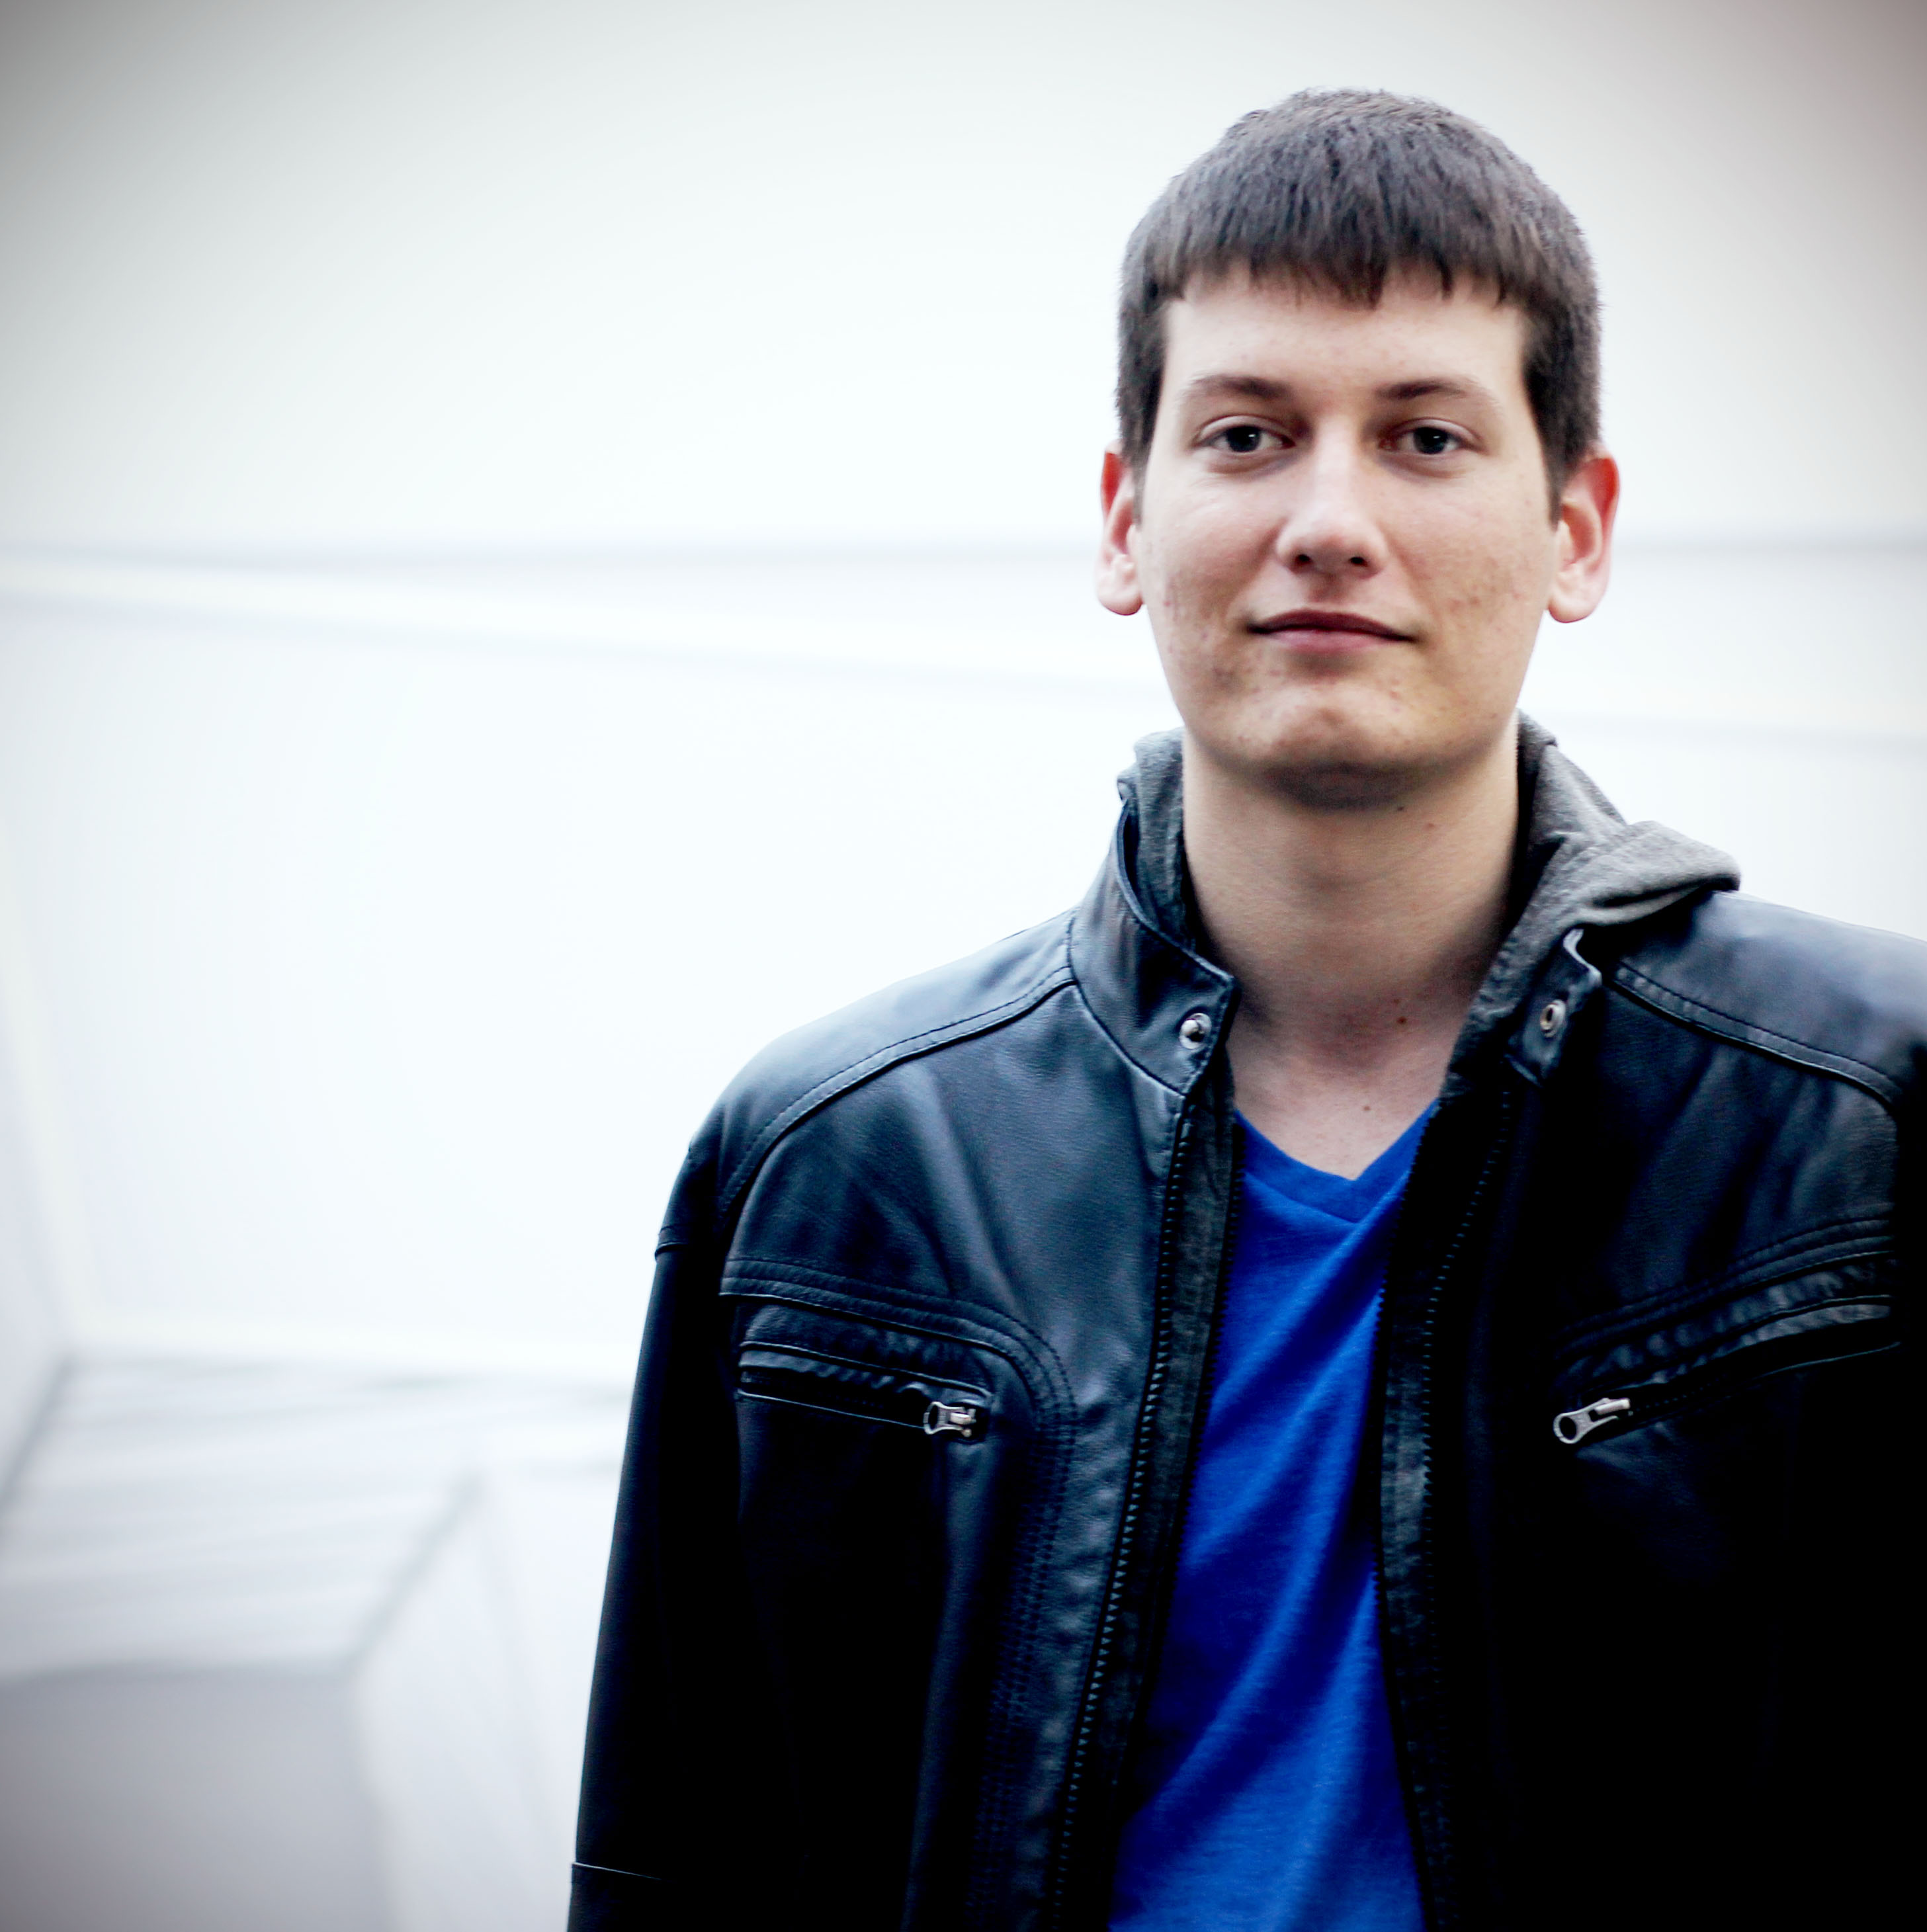
\includegraphics[width=0.25\textwidth]{img/group/josh}
  \end{center}
  \vspace{-20pt}
\end{wrapfigure}
Joshua Hillen is currently a third year student of computer science at the University of Toronto Scarborough campus. He is specializing in software engineering and plans to join the industry in 2015 directly after he graduates with an Honours Bachelor of Science. Previously to Joshua's current term he has learned and mastered a few languages, most importantly Java and C. He also participated in a group project where he was introduced to agile development and constructed software that modified .csv files for excel spreadsheets. Joshua has also taken on a variety of solo programming projects including an implementation of the Tiling Algorithm and the game Battleship. In his first two years Joshua's studies have primarily required critical thinking and time management; two important skills for group based work. He has broadened his perspective through electives including philosophy, psychology and astronomy. Joshua is a well rounded individual who has traveled overseas to Prague, Vienna, Budapest and South Africa.\\


\begin{wrapfigure}{l}{0.25\textwidth}
  \vspace{-20pt}
  \begin{center}
    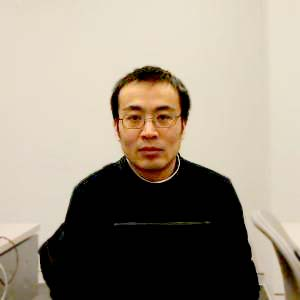
\includegraphics[width=0.25\textwidth]{img/group/kevin}
  \end{center}
  \vspace{-20pt}
\end{wrapfigure}
Yunqin Huang is a 4th year student of computer science in University of Toronto at Scarborough. He was born in China, and he spent his childhood there before he moved to Canada. His first language is Mandarin, and English is his second language, but he is proficient in both. He is not a very talkative person, and loves reading. He is experienced in C, Java, Python, and shell script, and quite familiar with UNIX platform. He has worked as a developer of applications on Solaris and Linux system in a network security company, and a developer of java EE web application in Medical service company.
He loves computer games and movies as well. \\

\begin{wrapfigure}{l}{0.25\textwidth}
  \vspace{-20pt}
  \begin{center}
    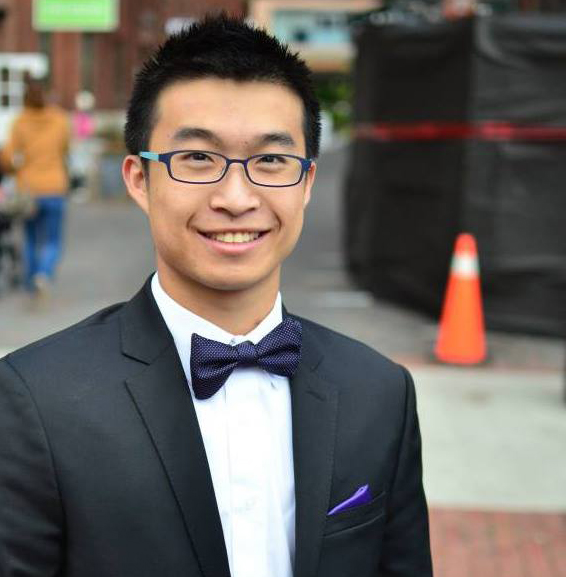
\includegraphics[width=0.25\textwidth]{img/group/derek}
  \end{center}
  \vspace{-20pt}
\end{wrapfigure}
Derek Lai was born in Hong Kong and came to Canada at the young age of 2. Ever since he was a kid, he has always wanted a job revolving around technology. Derek attended Unionville High School where he was first introduced to programming in Grade 9, learning his first programing language; Turing. From there, he furthered his computer science knowledge, learning both Visual Basic and Java. Derek is also the former President of his high school?s Robotics Team. Derek Lai is now currently a student at the University of Toronto working towards becoming a Software engineer. If not at school, he can usually be found in front of his computer or out with friends chatting over a cup of coffee.\\

\begin{wrapfigure}{l}{0.25\textwidth}
  \vspace{-20pt}
  \begin{center}
    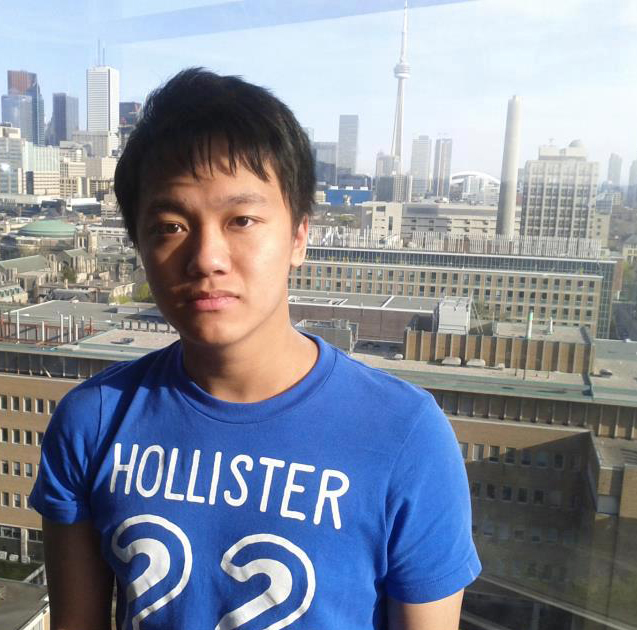
\includegraphics[width=0.25\textwidth]{img/group/dave}
  \end{center}
  \vspace{-20pt}
\end{wrapfigure}
Wei Hang was born in ZhanJiang, China December 27,1993. Wei Hang is prefer to be called Dave. Dave moved to Toronto, Canada at age of 9, studied and graduated from local elementary, and high school. He's a third year student studying at University of Toronto, Scarborough, estimated graduation date: 2014. In his spare time, he likes to play computer games such as League of Legend, Defence of the Ancient, Candy Crush, and Star Craft. Aside from his passion for video games, he also likes to study for fun. He loves to help people around him, sometimes he helps classmates with homework questions, and sometimes he volunteers to be a class note taker. Dave is planning to continue his graduate studies at University of Toronto st.George perusing degree in Master of Science. Dave is very passionate about programming and food, he would just sit on a chair and program for hours with a bag chips on the table, which explains why he's such a fatty! \\

\begin{wrapfigure}{l}{0.25\textwidth}
  \vspace{-20pt}
  \begin{center}
    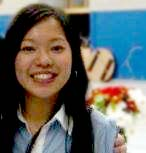
\includegraphics[width=0.25\textwidth]{img/group/candy.jpg}
  \end{center}
  \vspace{-20pt}
\end{wrapfigure}
Candy(Choi) Tak is currently a 4th year student at the University of Toronto, specializing in software engineering stream of computer science. She was born and raised in Hong Kong with 3 different languages, Cantonese, Mandarin and English. Also she is learning Korean as her 4th language. Candy decided to apply computer science after taking a programming course in high school.  She has experienced in Python, C, Java, and shell script as she study along with the terms. Candy also participated in few group projects. The Hackathon Hub is one of the projects that she enjoyed the most with agile development from the course Introduction to Software Engineering (CSC301). She specifically enjoys working on the front end and web developing, so she had chosen to take the design of Interactive Computational Media (CSCC318) as an elective, and hoping to continue with it after she graduates.\\

\section{matplotlib}

matplotlib is a plotting library that produces quality graphics for 2D(full support) and 3D(limited support) diagrams in Python. The library is most popular in the community for Python-based scientific computing  and can be applied in many different applications. matlplotlib comes with an interactive shell that can generate figures via simple python scripts, this includes the iPython shell embedded in MATLAB, IDL, or Mathematica. 

In addition, matplotlib is cross-platform compatible and can be embedded within web application servers and via any of the six GUI interface toolkits within different environments. These produce quality graphics in hardcopy that may be used for publication on the web or on paper. Supported formats include raster based graphics (PNG) and vector based graphics (PDF, PS, SVG). matplotlib can be used by a large range of users, from beginners who can use simple python commands, to power users who have full access to styling and graphical properties. A few examples of figures produced by matplotlib are illustrated in Figure~\ref{fig:examples}.

\begin{figure}
        \centering
        \begin{subfigure}[b]{0.3\textwidth}
                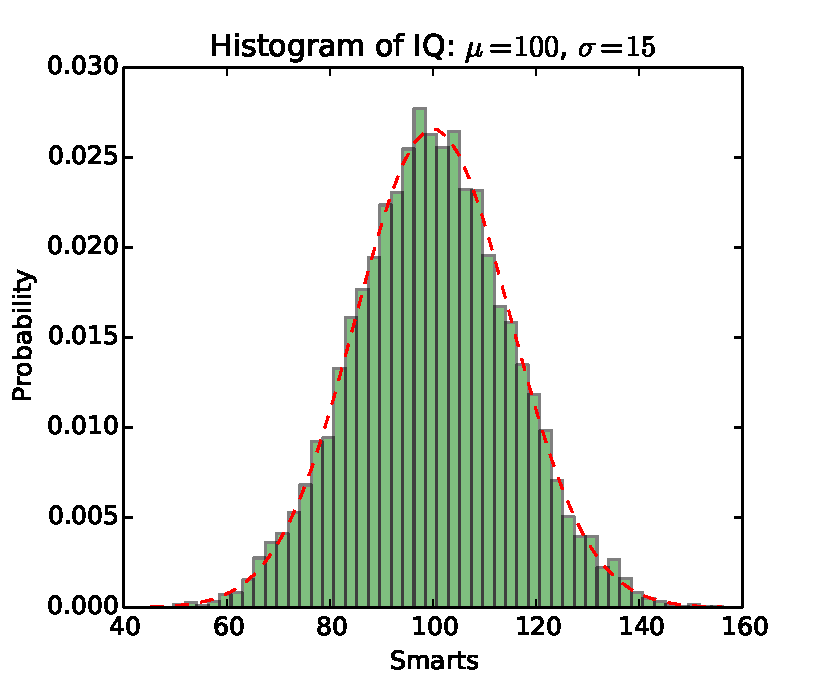
\includegraphics[width=\textwidth]{img/examples/histogram}
                \caption{Histogram example}
                \label{fig:histogram}
        \end{subfigure}%
        ~ %add desired spacing between images, e. g. ~, \quad, \qquad etc.
          %(or a blank line to force the subfigure onto a new line)
        \begin{subfigure}[b]{0.3\textwidth}
                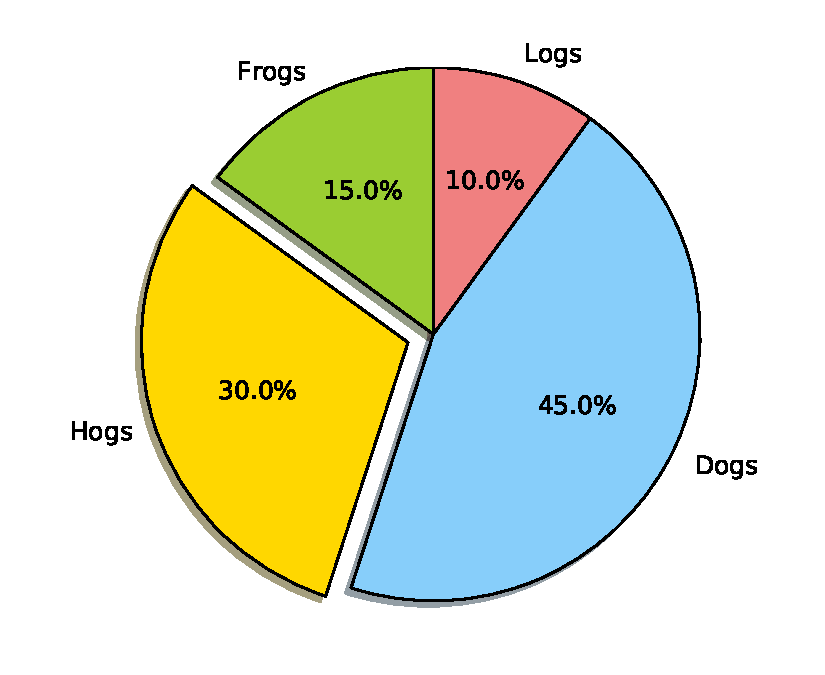
\includegraphics[width=\textwidth]{img/examples/pie}
                \caption{Pie chart example}
                \label{fig:pie}
        \end{subfigure}
        ~ %add desired spacing between images, e. g. ~, \quad, \qquad etc.
          %(or a blank line to force the subfigure onto a new line)
        \begin{subfigure}[b]{0.3\textwidth}
                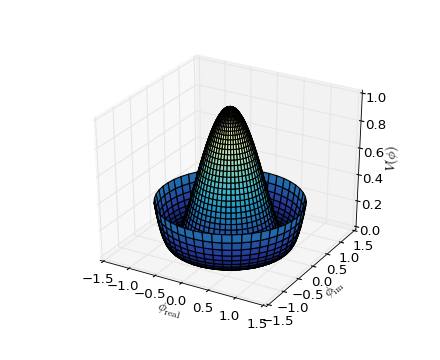
\includegraphics[width=\textwidth]{img/examples/mplot3d}
                \caption{mplot3d toolkit example}
                \label{fig:mplot3d}
        \end{subfigure}
        \caption{Examples of matplotlib graphics}\label{fig:examples}
\end{figure}



%xxxxxxxxxxxxxxxxxxxxxxxxxxxxxxxxxxxxxxxxxxxxxxxxxxxxxxxxxxx
%xxxxxxxxxxxxxxxxxxxxxxxxxxxxxxxxxxxxxxxxxxxxxxxxxxxxxxxxxxx

\chapter{The Process}

\section{Reverse Engineering Tools}

Our group decided to find a suitable reverse engineering tool to aid us in generating a UML class diagram that represents all the classes, subclass relationships, and associations in the source code. We initially took a look at various applications that would provide us with the necessary tools to generate diagrams from the matplotlib source code. Some of these applications included visual paradigm, pywebuml, pyreverse, etc. 

We initially looked at pyreverse. There were two obvious problems, firstly even panning through the diagram it produced was very slow, and secondly it only exported to graphviz dot files, which had no good graphical editors. Having a good graphical editor was quite important as we needed to remove unnecessary detail and split up the diagrams, so we began to look at alternatives. Unfortunately we could not find any open source software that had a good graphical editor and python reverse engineering, so we moved into trial versions of commercial software. We started with Visual Paradigm for UML. The reverse engineering and graphical editor were good, and it was also cross platform, but the produced diagram was still very cluttered and complicated as can be seen in Figure~\ref{fig:vp}. The reverse engineering of VP was nice, but the resulting diagram was cluttered and confusing.

\begin{figure}[ht!]
        \centering
                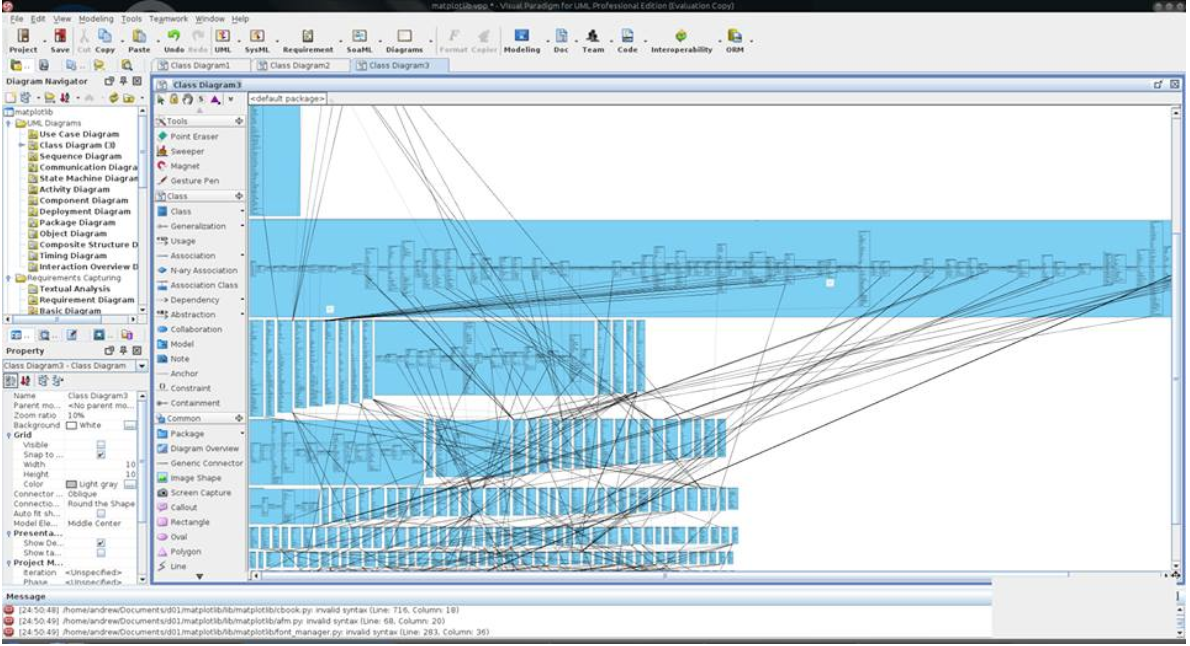
\includegraphics[width=0.5\textwidth]{img/process/vp}
        \caption{Visual Paradigm's output from matlplotlib sourcecode}\label{fig:vp}
\end{figure}

We next looked at Enterprise Architect (EA). It had a nice clean interface, and most importantly, was quick and produced a very organized and easy to split diagram from reverse engineering. The result can be seen in Figure~\ref{fig:ea}. The diagram produced by EA was much more organized and easy to read.

\begin{figure}[ht!]
        \centering
                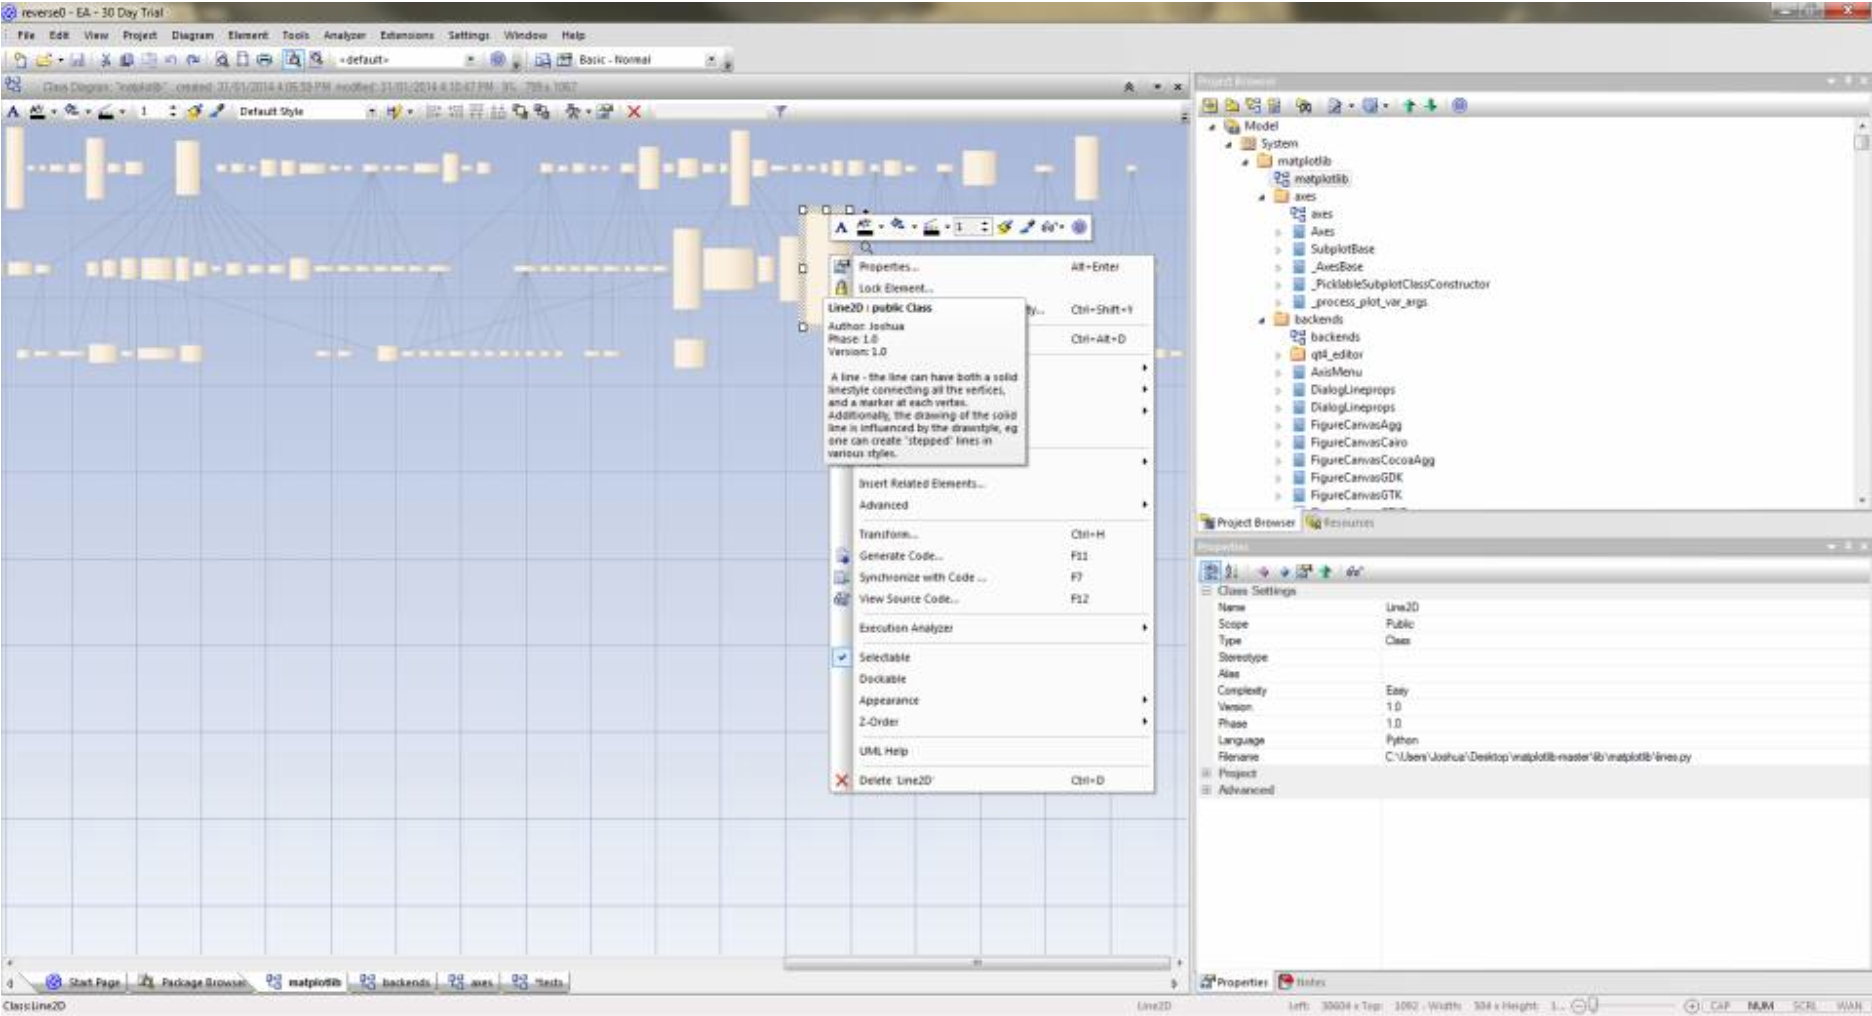
\includegraphics[width=0.5\textwidth]{img/process/ea}
        \caption{Enterprise Architect's output from matlplotlib sourcecode}\label{fig:ea}
\end{figure}

After listing and analyzing some of the pros and cons of each application, we unanimously agreed on Enterprise Architect by Sparx Systems (Sparx). Many of the applications offered us a way to input our matplotlib source code and return a UML class diagram representing all the relationships within it. However since we still needed to edit the generated model to capture information missed by the tool, and remove unnecessary details, we found Sparx provided us a way to do this with ease.


\section{Abstraction Steps}

After generating our initial model from the raw source code, we split up the diagram into even parts that we could all simplify and understand. This allowed us to work in parallel which is helpful when tackling such a large codebase. We were supposed to identify important modules and relationships while simplifying the models so that we could get a better understanding of the higher abstractions of the system. Because Enterprise Architect has a very clear tree model, it helped us quickly identify important abstractions, as they were often parents of a large tree.

Reflecting back on this though, it was perhaps not the best method. Because we each only had a small part of the whole library, none of us could get a great overview of the whole system. While it was still somewhat effective, because each of us only knew a small portion of classes we couldn?t visualize the proper relationships between major classes. 

What eventually ended up really helping us get a proper high level picture of matplotlib was the Architecture of Open Source Applications article (\url{http://aosabook.org/en/matplotlib.html}) written by the founder of matplotlib John Hunter. Once we read through that document we gained a much better understanding of the general architecture of matplotlib and the motivations behind certain design decisions. After also looking at the matplotlib docs (\url{http://matplotlib.org/contents.html}) and checking the matplotlib init.py file to see the bigger picture we were much more easily able to identify important components and relationships. In hindsight, it would have been better if we could have gotten a good overview first, and then split up the uml. It would have allowed us to split up the diagram more effectively and keep relevant classes and relationships together.



%xxxxxxxxxxxxxxxxxxxxxxxxxxxxxxxxxxxxxxxxxxxxxxxxxxxxxxxxxxx
%xxxxxxxxxxxxxxxxxxxxxxxxxxxxxxxxxxxxxxxxxxxxxxxxxxxxxxxxxxx

\chapter{System Architecture}

\section{Overview}

One of matplotlibs main functionalities is to create a framework that will manipulate, render, and represent the Figure object. A Figure in matlplotlib is a top-level object (derived from an Artist, as explained below) that encapsulates all the various lines, axis, lines, curves, etc. An advantage in matplotlibs framework is that it has decoupled the aggregation on Figure away from its rendering onto an output source (hardcopy, GUI, etc). By doing so, this allows matplotlib to extract the backend and user/output layer away from the heavy duty Figure logic and calculations. This has also enabled developers to incorporate event handling via user mouse and keyboard by just extending / adding plugins without needing to modify the existing source and supported toolkits. 

\subsection{Strengths \& Weaknesses}

matplotlib achieves this architecture by separating it's components into three distinct layers, Backend Layer (bottom), Artist Layer (middle), and Scripting Layer (top) as seen in Figure~\ref{fig:threeTier}. The three layers are designed as a closed system architecture, which aids in minimizing dependencies between the layers and reduces the impact of future change (for example, it is easy to add new backends without modification elsewhere). Since the scripting layer and the backend layer are independent of each other, it allows them to be more modifiable. In addition, keeping the rendering (from the backend) segregated, allows the user to {\it write once, run anywhere}.

Unfortunately there are some drawbacks to the matplotlib codebase being, every graphical output is an instance of an artist. This means a lot of unnecessary data and methods are inherited by all these classes which may never use them. The artist abstract class (discussed later on in the Artist layer) has become significantly large. In addition to the artist, many of matplotlib's classes are colossal.



\begin{figure}[ht!]
        \centering
                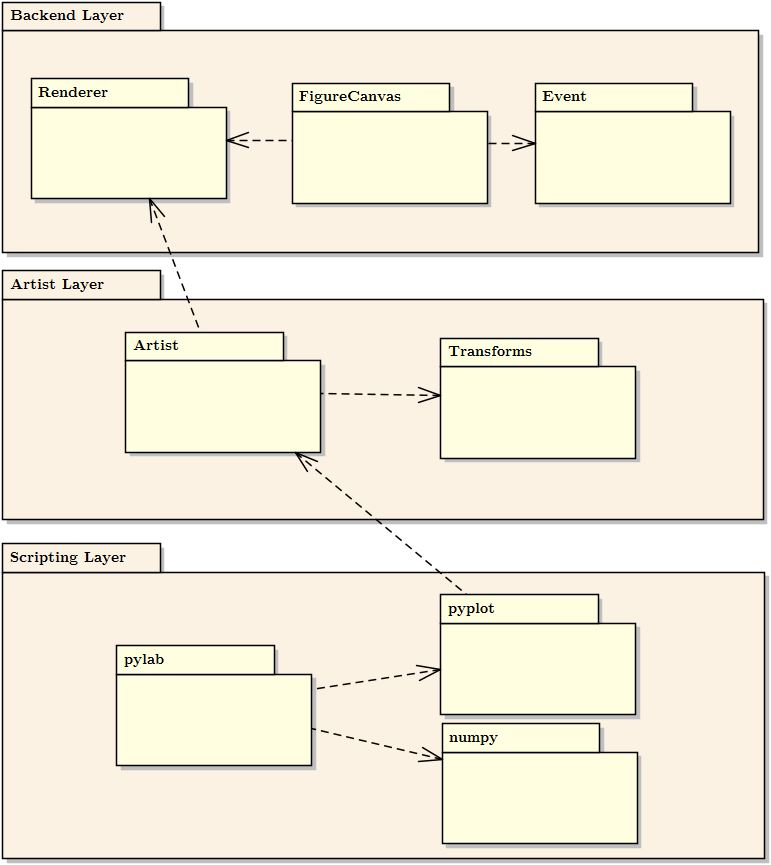
\includegraphics[width=0.5\textwidth]{img/umls/arch/threeTierArch.jpg}
        \caption{3-Tiered Architecture of matlplotlib}\label{fig:threeTier}
\end{figure}

%----------------------------------------------------------------------------------------
\section{Backend Layer}

The matplotlib backend layer is the coupling between the specific graphics toolkits and the generic APIs used by the Artist layer. Currently matplotlib supports multiple backends including GTK, Qt, Tk, and Wx. In order to prevent direct dependencies there are three main abstract components of the backend layer, the FigureCanvas, the Renderer and the Event. Each toolkit must provide concrete implementations of these classes.

\subsection{FigureCanvas}

The FigureCanvas is analogous to a sheet of paper to be drawn on. It handles the specifics of setting up either the GUI window or image file for the Renderer to draw into. It also handles the events on these windows and converts them to a form based on the matplotlib Event classes. For example if the user moves their mouse wheel over the display window then the FigureCanvas receives a Qt wheelEvent and converts it to matplotlib MouseEvent and dispatches it.

\subsection{Renderer}
The Renderer maps the generic matplotlib draw commands to the specific commands of the toolkit implementation. For instance the Renderer method draw\_path calls the underlying wx DrawPath or StrokePath methods. The main methods required in Renderer are draw\_path, draw\_image, and draw\_text. A high performance C++ library, AGG (Anti-Grain Geometry), is a Renderer backend that has proven to work well across platforms and GUIs.

\subsection{Event}
The Event framework handles underlying UI events. Toolkit specific keyboard and mouse events are converted to matplotlib KeyEvent or MouseEvent classes. Listeners can be bound to these events to provide rich user interactions. By mapping the UI specific events to generic Event classes, matplotlib is able to provide a consistent user experience across UIs.

\subsection{Strengths and Weaknesses}
It is clear that matplotlib has a decoupled approach to the backend layer. Events are converted to generic classes, and Renderers only need to implement a handle of functions: draw\_path, draw\_image, draw\_text, and get\_text\_width\_height\_descent. There are advantages and disadvantages to this approach. For one it makes it very easy to add support for a new backend; and a change in the underlying toolkits would require only minor refactoring. In addition, from the user's perspective, it provides a wide variety of toolkits that can be easily interchanged. On the other hand using such a generic interface prevents specialized optimizations. Matplotlib mitigates this somewhat by providing additional optional APIs such as draw\_markers, draw\_path\_collection, and draw\_quad\_mesh. These methods are much more efficient than just using draw\_path, but only certain toolkits support them. By using such a compact API matplotlib cannot utilize the specific optimizations of each toolkit. It takes the approach of jack of all trades, master of none. Considering the open source nature of matplotlib though, this flexibility is probably the preferable design decision.

%----------------------------------------------------------------------------------------
\section{Artist Layer}

Proceeding the top-level backend layer, we have matplotlib's Artist Layer. As the middle tier in the closed 3-layered architecture, the Artist Layer has the responsibility of connecting the Scripting Layer to the Backend Layer(see Figure~\ref{fig:threeTier}). 

\subsection{Artist}
\begin{figure}[ht!]
        \centering
                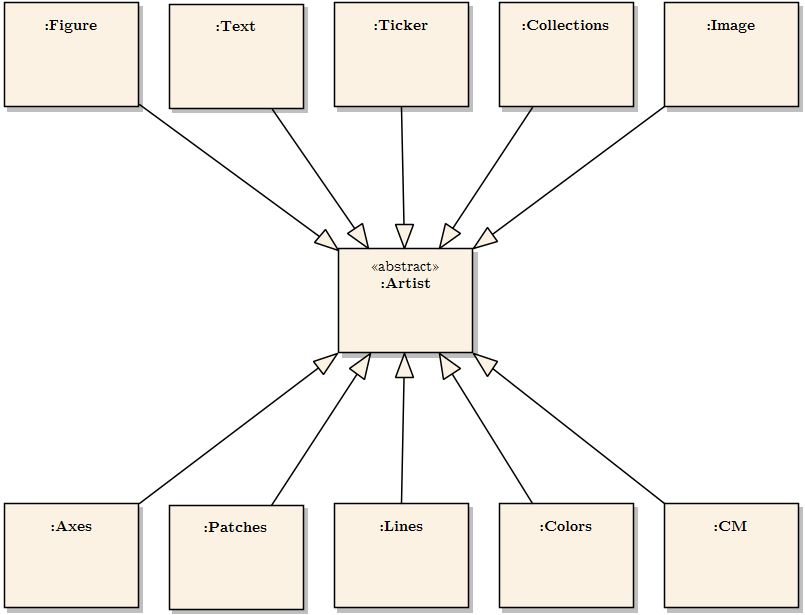
\includegraphics[width=0.5\textwidth]{img/umls/arch/absArtist}
        \caption{Derivations from the abstract Artist class}\label{fig:absArtist}
\end{figure}
The Artist Layer contains one of matlplotlib's core abstract classes, the Artist. This class is what takes the Renderer and places the intended graphics onto the FigureCanvas. Every component we see in the final graphic is a concrete instance of the Artist class. Figure~\ref{fig:absArtist} only shows 10 main modules that were derived from the artist class. Detailed descriptions and class diagrams of each module can be found below. For now let's look at a simple example of how the Artist instances are used in Figure~\ref{fig:artistEx} from matplotlib's gallery.

\begin{figure}[ht!]
        \centering
                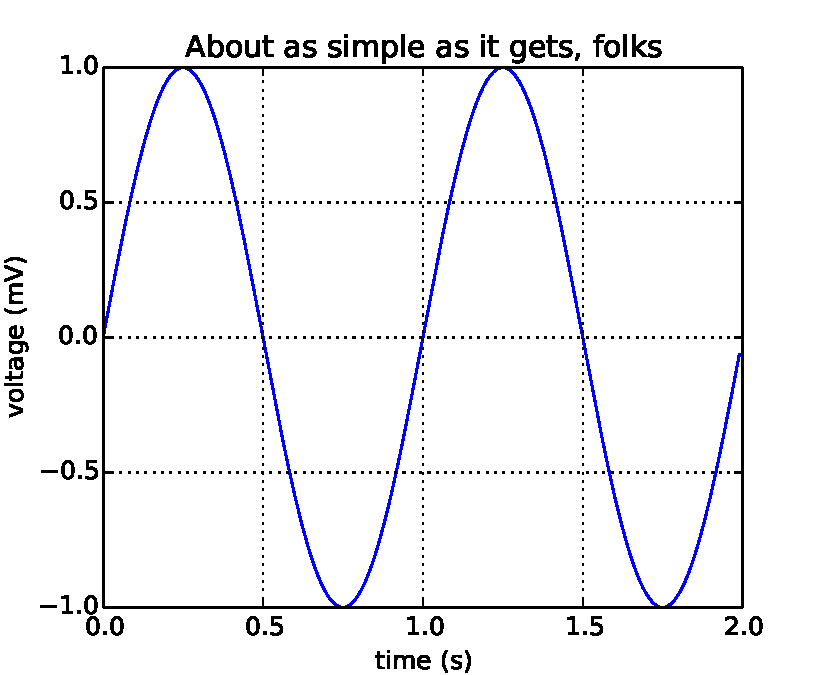
\includegraphics[width=0.3\textwidth]{img/examples/simple_plot}
        \caption{Hierarchy of the artist instances used to draw Figure~\ref{fig:artistExAgg}}\label{fig:artistEx}
\end{figure}

We must first divide the abstract Artist into two separate categories, primitive and composite. The primitive artists are standalone instances of artists like Text, Line2D (sine line), shapes, etc. A composite artist is one that holds a multitude of primitive and other composite artist instances. The first instance created is the Figure instance, a composite artist which contains one of matplotlib's major composite artists, the Axes. The Axes encapsulates all the artist instances that follow, including the Title, Axes, Labels, Ticks, etc. Fig~\ref{fig:artistExAgg} shows a partitioning hierarchy of Figure~\ref{fig:artistEx} was created.

\begin{figure}[ht!]
        \centering
                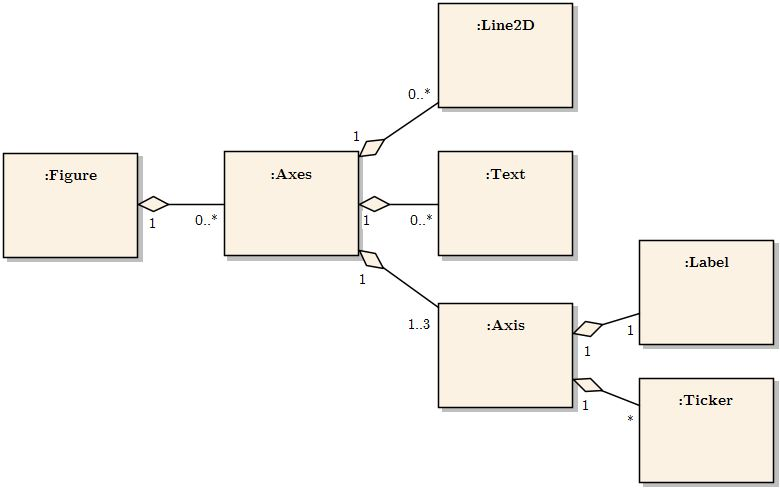
\includegraphics[width=0.5\textwidth]{img/umls/arch/artistExAgg}
        \caption{3-Tiered Architecture of matlplotlib}\label{fig:artistExAgg}
\end{figure}

We know the coupling between the Artist Layer and the Backend Layer happens via the Artist and Renderer instances. Specifically, the draw method inside artist must call a suitable method from the Renderer's API (e.g. draw\_path, draw\_image, and draw\_text). Below is the abstract draw method from the abstract Artist class.


\begin{lstlisting}
def draw(self, renderer, *args, **kwargs):
        '''Derived classes drawing method'''
        if not self.get_visible():
            return
\end{lstlisting}

An example of how this method is implemented in a derived artist class, such as Line2D is provided below.

\begin{lstlisting}
def draw(self, renderer, gc, path, trans):
        '''Simplified example from Line2D class'''
        if not self.get_visible():
            return
        renderer.draw_path(gc, path, trans)
\end{lstlisting}

\subsection{Transforms}

From the above implementation of draw in Line2D we see that a variable trans is used. This variable is an instance of Transform. Inside the Artist Layer, lies a package for Transformations, which is essentially a tool to map coordinates from one system to another (e.g. raw data, axes, figure, display). Transform node is shared attribute among all Artists, and is thus, part of the abstract Artist class. 
\begin{lstlisting}
    def set_transform(self, t):
        '''Set the :class:`~matplotlib.transforms.Transform` instance
       used by this artist.

       ACCEPTS: :class:`~matplotlib.transforms.Transform` instance'''
        self._transform = t
        self._transformSet = True
        self.pchanged()
\end{lstlisting}

Other shared attributes among artists include, the visibility, labels, if animated, the picker (detects user mouse clicks), etc.

\subsection{Strengths and Weaknesses}


%----------------------------------------------------------------------------------------
\section{Scripting Layer}

The scripting layer is a high level interface that allows for non-programmers to more easily work with matplotlib. It handles a lot of the boilerplate allowing for users such as scientists to more quickly and easily plot their data. The main module for this is the pyplot module, and it has intuitive commands that significantly simplify scripts. For example the standard artist code:

\begin{lstlisting}
from matplotlib.backends.backend_agg import FigureCanvasAgg as FigureCanvas
from matplotlib.figure import Figure
fig = Figure()
canvas = FigureCanvas(fig)
x = np.random.randn(10000)
ax = fig.add_subplot(111)
ax.hist(x, 100)
ax.set_title('Normal distribution with $\mu=0, \sigma=1$')
fig.savefig('matplotlib_histogram.png')
\end{lstlisting}
as been reduced to:

\begin{lstlisting}
import matplotlib.pyplot as plt
import numpy as np
x = np.random.randn(10000)
plt.hist(x, 100)
plt.title(r'Normal distribution with $\mu=0, \sigma=1$')
plt.savefig('matplotlib_histogram.png')
plt.show()
\end{lstlisting}


Hiding the concepts of figures and canvas and providing the central plt object to handle all of the calls makes it much easier for the average user to understand and use.
In addition to reducing code for the user, matplotlib has ensure that pyplot does not add significant code behind the scenes. By using the $@$docstring.copy\_dedent annotation and passing args to the underlying Artist functions via \*args and \*\*kwargs, pyplot is able to replicate functionality of many Artist classes without much duplication. For example the savefig method looks like this:

\begin{lstlisting}
@docstring.copy_dedent(Figure.savefig)
def savefig(*args, **kwargs):
	fig = gcf()
	res = fig.savefig(*args, **kwargs)
	draw()   # need this if 'transparent=True' to reset colors
	return res
\end{lstlisting}

This design allows the scripting layer to effectively reproduce Artist behaviour while creating minimal new logic. Changes in the underlying Artists should require minimal refactoring in the scripting layer. This can occasionally be a weakness as well though. Since the scripting layer is essentially just forwarding to the artist layer, changes in the artist layer will cause changes in the scripting syntax, this can be seen as undesirable if users old scripts all of a sudden stop working with a certain version.

%----------------------------------------------------------------------------------------
\chapter{Matplotlib In-Depth}

Below are more detailed class diagrams and descriptions of the main individual components inside matplotlib. 

%S1--------------------------------------------------------------------------------------
\subsection{Tranforms}
Transforms are a crucial part of matplotlib, and handle everything from zooming in and out, to changing coordinate systems. Every transform is made up of a tree of TransformNode objects, and these can either be transformations or the bounding boxes for those transformations.
\begin{figure}[ht!]
        \centering
        \begin{subfigure}[b]{0.4\textwidth}
                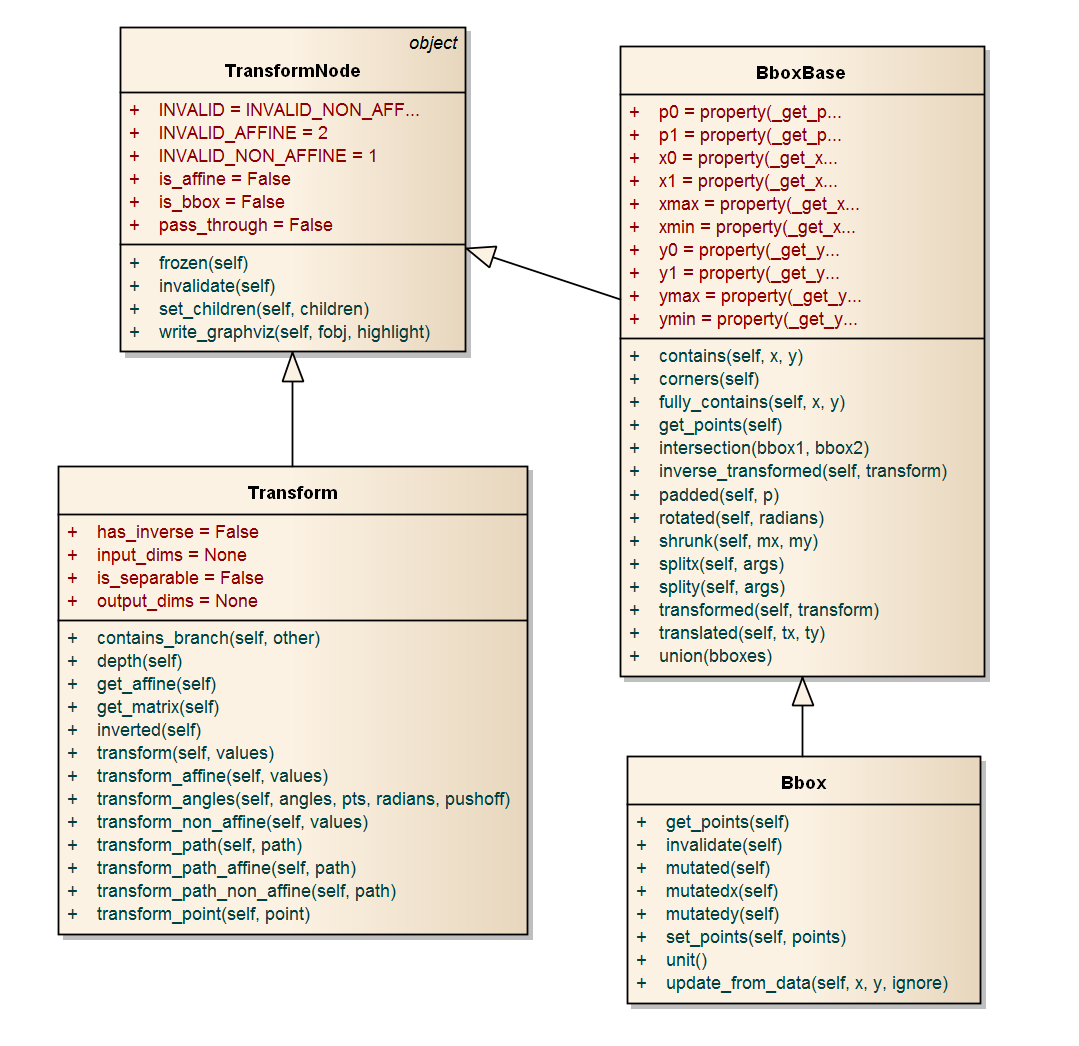
\includegraphics[width=\textwidth]{img/umls/andrew/transformNode}
                \caption{}
                \label{fig:transform1}
        \end{subfigure}%
        ~ %add desired spacing between images, e. g. ~, \quad, \qquad etc.
          %(or a blank line to force the subfigure onto a new line)
        \begin{subfigure}[b]{0.4\textwidth}
                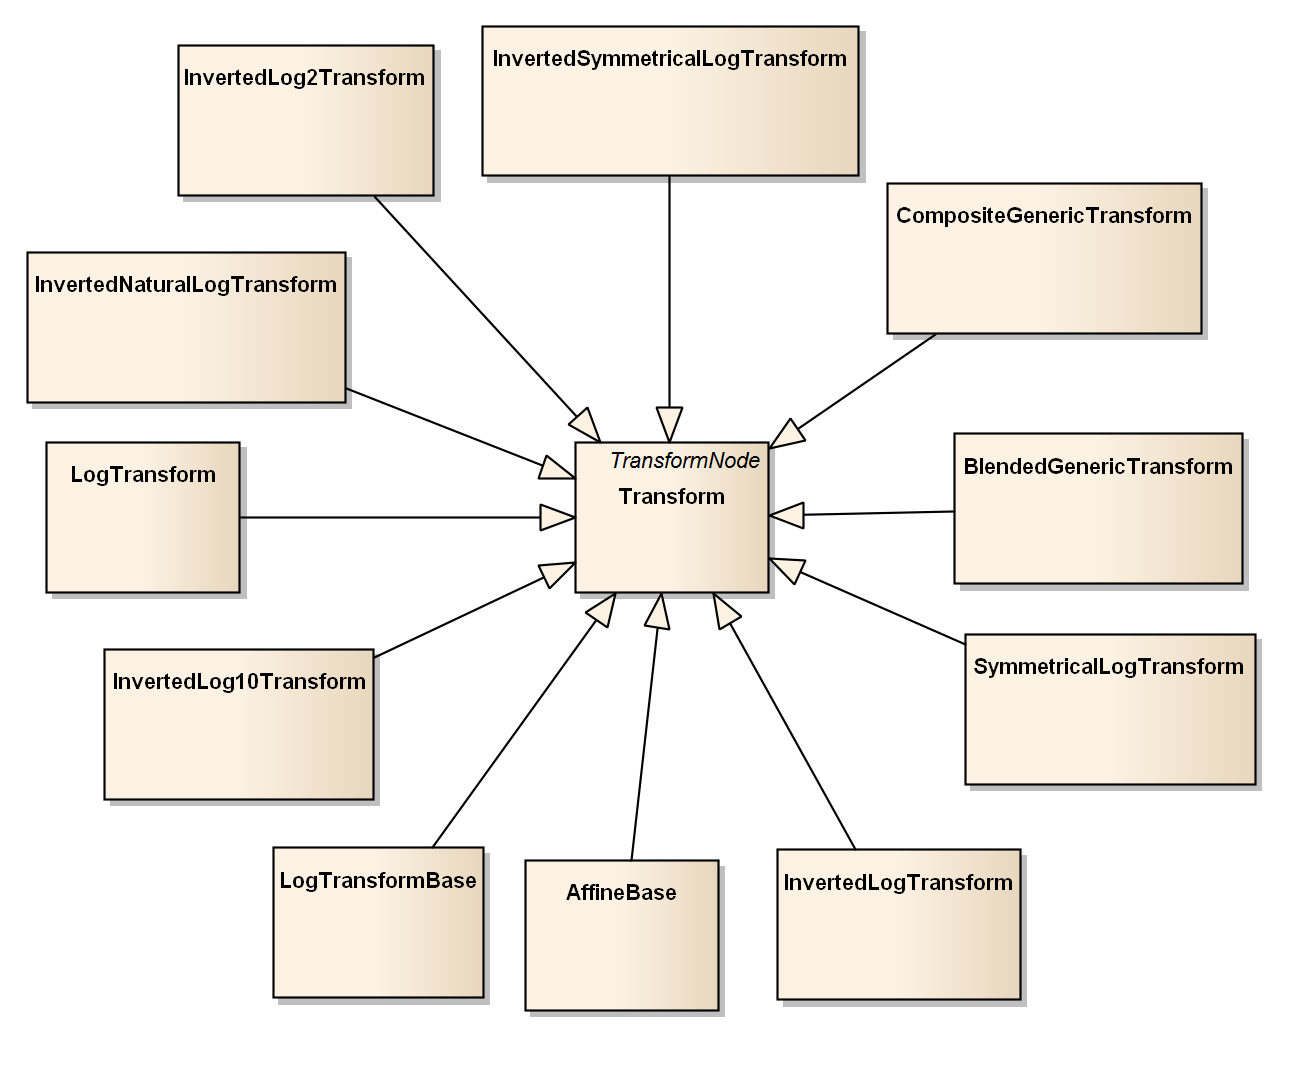
\includegraphics[width=\textwidth]{img/umls/andrew/transform}
                \caption{}
                \label{fig:transform2}
        \end{subfigure}
        \caption{TransformNode's class diagrams}\label{fig:examples}
\end{figure}

Figure~\ref{fig:transform1} is the main TransformNode parent which the transforms extend. Figure~\ref{fig:transform2} shows the same Transform class with it at the centre and all the default transformations surrounding it, including AffineBase, which handles standard transformations such as panning, zooming, and rotation as well as various logarithmic transforms. 
\begin{figure}[ht!]
        \centering
                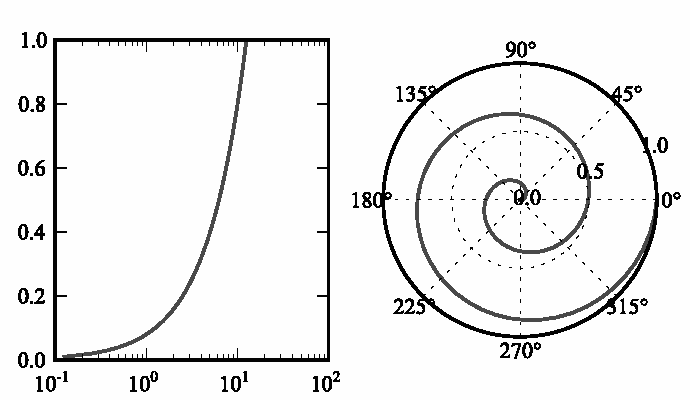
\includegraphics[width=0.3\textwidth]{img/umls/andrew/nonaffine_transforms}
        \caption{Graphical interpretations of logarithmic transforms}\label{fig:transform_demo}
\end{figure}
An example of the same data graphed using a logarithmic transform on the left and a polar transform on the right in Figure~\ref{fig:transform_demo}.


\subsection{Legend}
The Legend class is a child of Artist that encapsulates the functionality of drawing legends onto graphs, as can be seen in Figure~\ref{fig:legend_demo}.
\begin{figure}[ht!]
        \centering
                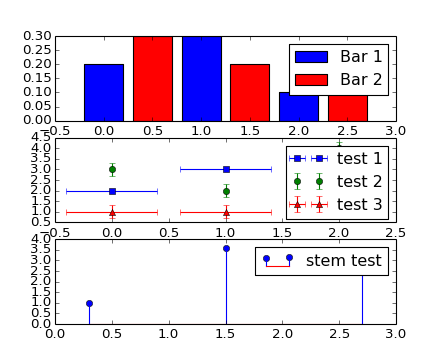
\includegraphics[width=0.3\textwidth]{img/umls/andrew/legend_demo}
        \caption{Three example graphs with legends on the top right.}\label{fig:legend_demo}
\end{figure}

The actual handling of drawing the legend is taken care of by the legend handler classes which extend the HandlerBase class. For example there are different handlers for patch type (rectangle, circle) graphs, point/dot graphs, and line graphs.
See Figure~\ref{fig:legend}  for relationship between the Legend and legend handler classes.
\begin{figure}[ht!]
        \centering
                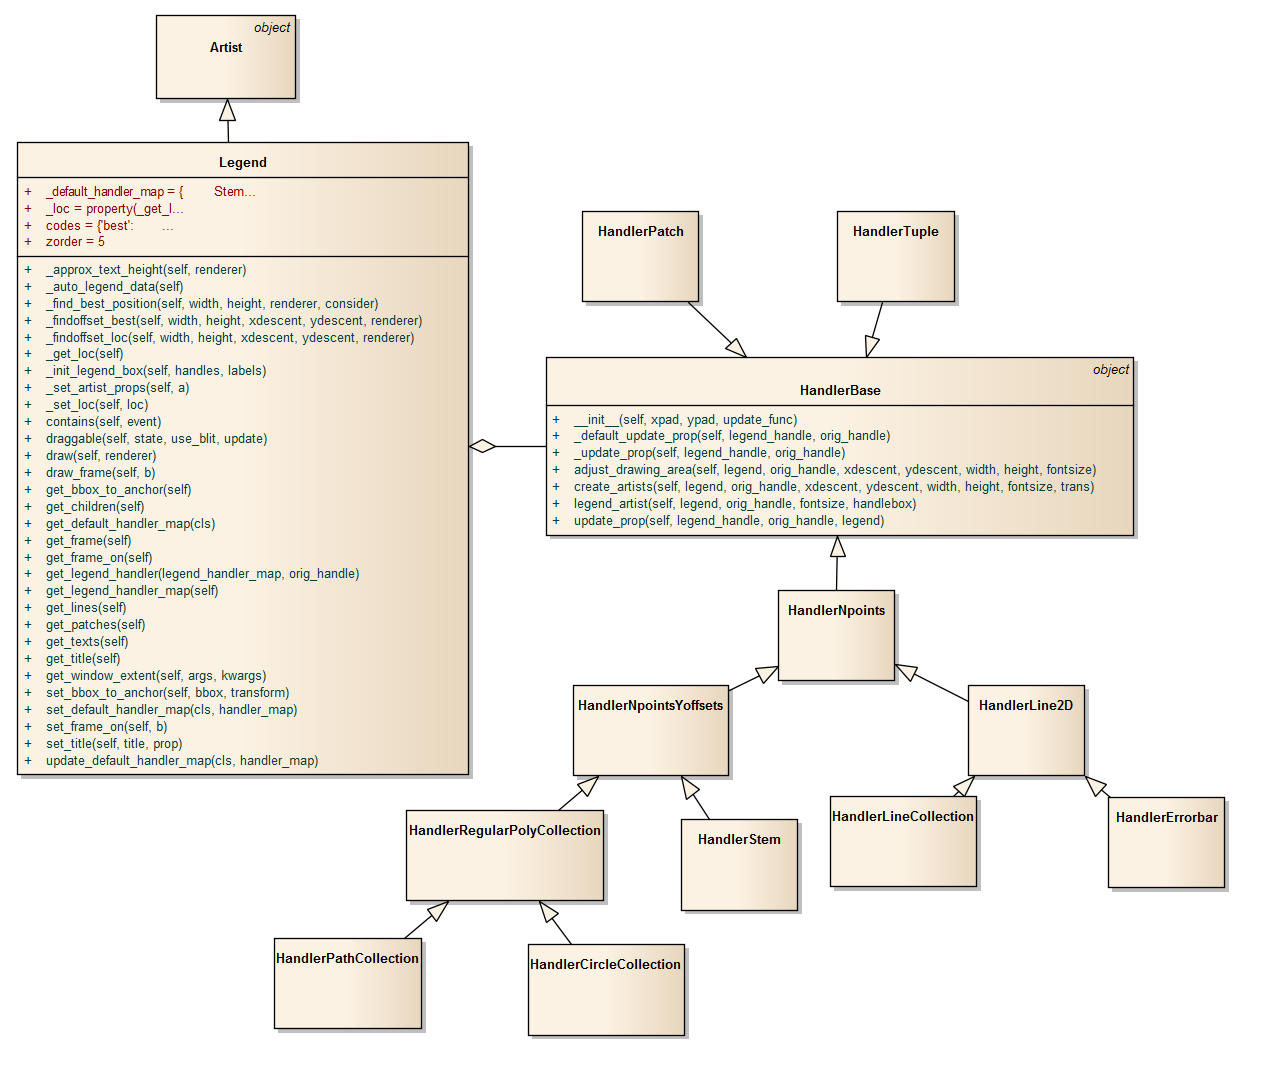
\includegraphics[width=0.55\textwidth]{img/umls/andrew/legend}
        \caption{Legend and LegendHandler}\label{fig:legend}
\end{figure}

%S3--------------------------------------------------------------------------------------

\subsection{Collections}

Collections is an abstract class derived from an Artist class. It is a composite type of artist which is used to group other artists of a similar type together into a collection. Derivations include LineCollection, PatchCollection, EllipseCollection and etc. (see Figure)

\begin{figure}[ht!]
        \centering
                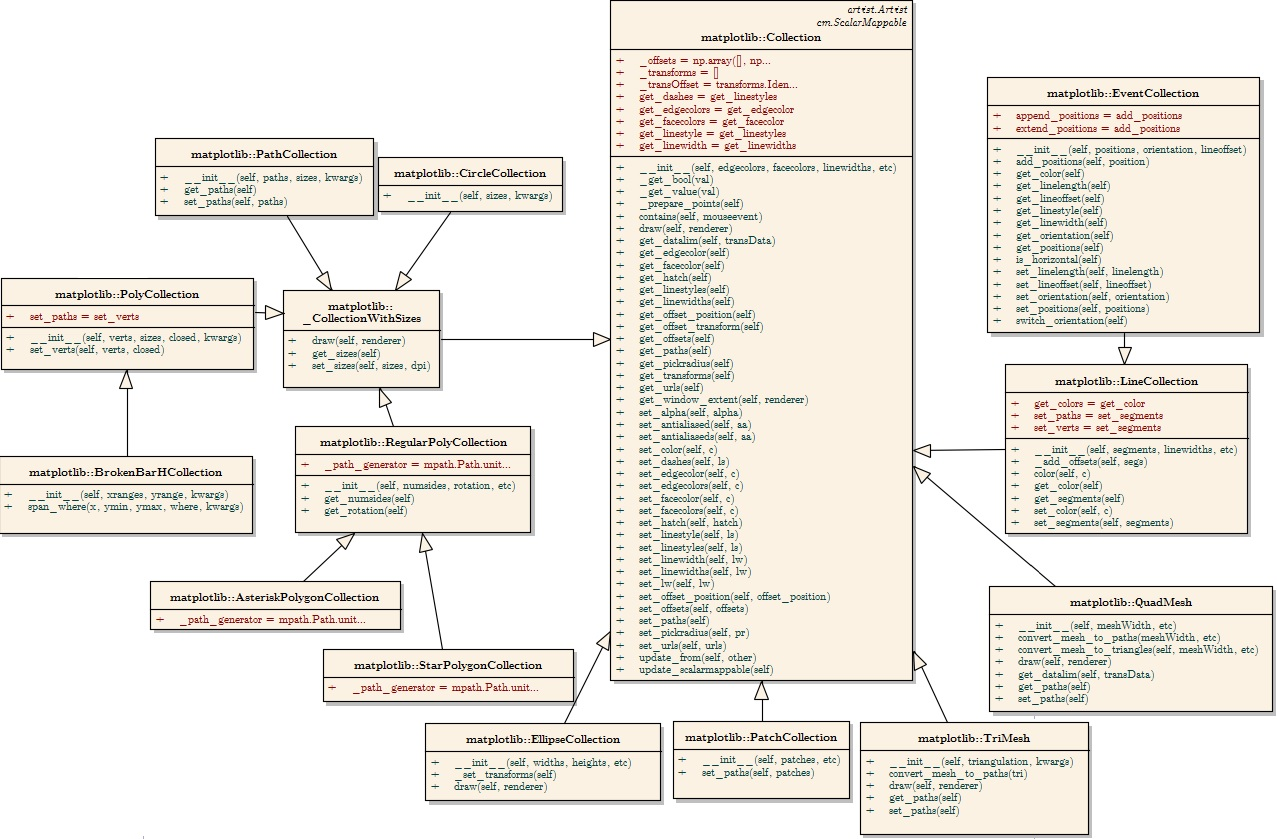
\includegraphics[width=0.5\textwidth]{img/umls/pi/collections}
        \caption{Collections and selected subclasses}\label{fig:artistExAgg}
\end{figure}

\subsection{Animation}
The animation class is an abstract class that wraps the creation of an animation. A subclass derived from it is TimedAnimation (supports time-based animation / drawing frames on an interval bases) which itself as derivations of ArtistAnimation and FuncAnimation (see Figure).

\begin{figure}[ht!]
        \centering
                \includegraphics[width=0.3\textwidth]{img/umls/pi/animation}
        \caption{Animation and selected subclasses}\label{fig:artistExAgg}
\end{figure}

\subsection{Ticker}
The Tick object is another abstract class derived from the abstract artist, used for the axis ticks, gridlines and labels. Both the XTick, and YTick classes are subclasses of Tick.The TickHelper is an abstract class that is used to create a Locator and Formatter for the Tick artists. The Locator determines the tick locations and has many child classes such as LogLocator, LinearLocator, FixedLocator, etc.  The formatter instance of TickHelper converts the tick locations into the strings and also has many child classes such as, ScalarFormatter, FixedFormatter, IndexFormatter, etc. to suit your needs (See Figure)

\begin{figure}[ht!]
        \centering
        \begin{subfigure}[b]{0.3\textwidth}
                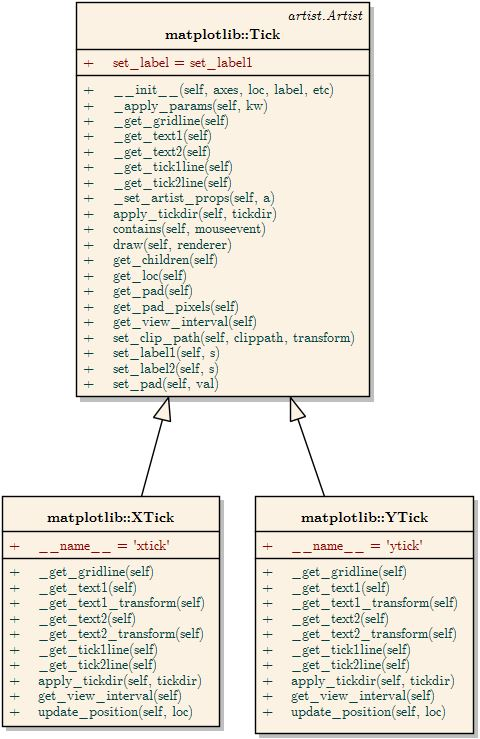
\includegraphics[width=\textwidth]{img/umls/pi/tick}
                \caption{Tick}
                \label{fig:histogram}
        \end{subfigure}%
        ~ %add desired spacing between images, e. g. ~, \quad, \qquad etc.
          %(or a blank line to force the subfigure onto a new line)
        \begin{subfigure}[b]{0.3\textwidth}
                \includegraphics[width=\textwidth]{img/umls/pi/tickhelper}
                \caption{TickHelper}
                \label{fig:pie}
        \end{subfigure}
        \caption{Tick classes which are used to draw ticks on the axes}\label{fig:examples}
\end{figure}


%S2--------------------------------------------------------------------------------------

\subsection{Event}

FigureCanvas encapsulates the idea of a drawing surface (e.g. the paper). For each user interface toolkit, there is a concrete implementation of FigureCanvas that derives from FigureCanvasBase which knows how to draw itself into a window, transfer renderer commands onto the canvas, and convert the toolkits events to matplotlibs Event class (see Figure).

\begin{figure}[ht!]
        \centering
                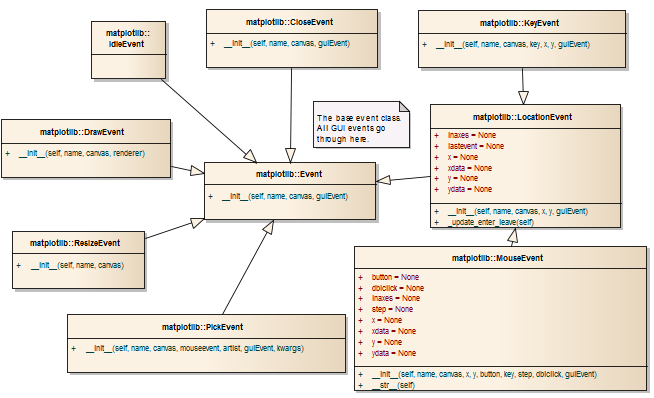
\includegraphics[width=0.6\textwidth]{img/umls/nick/event}
        \caption{The event classes and all of its subclasses}\label{fig:artistExAgg}
\end{figure}

\subsection{FigureCanvasBase}

FigureCanvasBase is the abstraction layer that separates the class matplotlib.figure.Figure from the backend specific details like a user interface drawing area. FigureCanvas encapsulates the idea of a drawing surface (e.g. the paper). For each user interface toolkit, there is a concrete implementation of FigureCanvas that derives from FigureCanvasBase which knows how to draw itself into a window, transfer renderer commands onto the canvas, and convert the toolkits events to matplotlibs Event class (see Figure).

\begin{figure}[ht!]
        \centering
                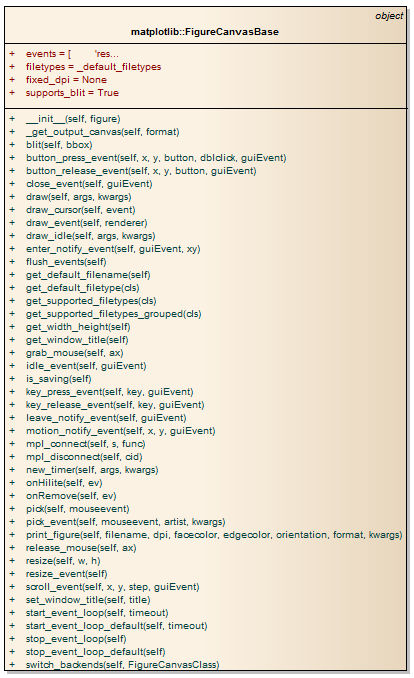
\includegraphics[width=0.3\textwidth]{img/umls/nick/figcanbase}
        \caption{The FigureCanvas abstract parent class}\label{fig:artistExAgg}
\end{figure}

%S4--------------------------------------------------------------------------------------
\subsection{Axes}
Transforms data into horizontally and vertically classed display coordinates (x,y).
\begin{figure}[ht!]
        \centering
                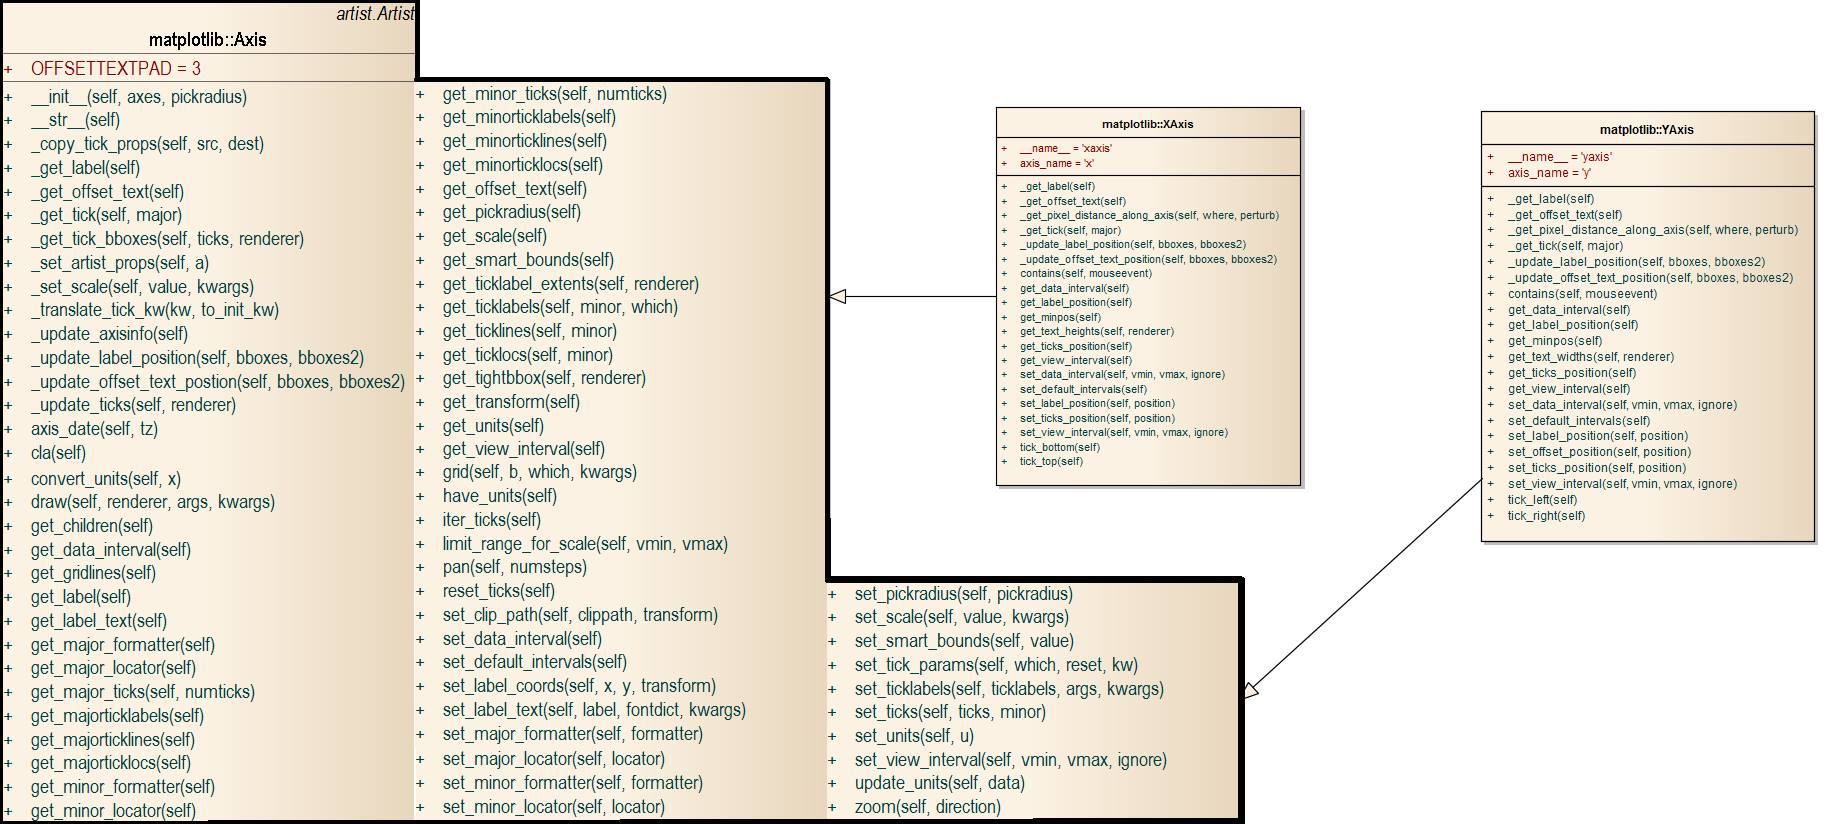
\includegraphics[width=0.8\textwidth]{img/umls/josh/axis}
        \caption{The Axis class and its subclasses}\label{fig:math text}
\end{figure}

\subsection{Image}
Responsible for transforming, displaying, creating and retrieving images.
\begin{figure}[ht!]
        \centering
                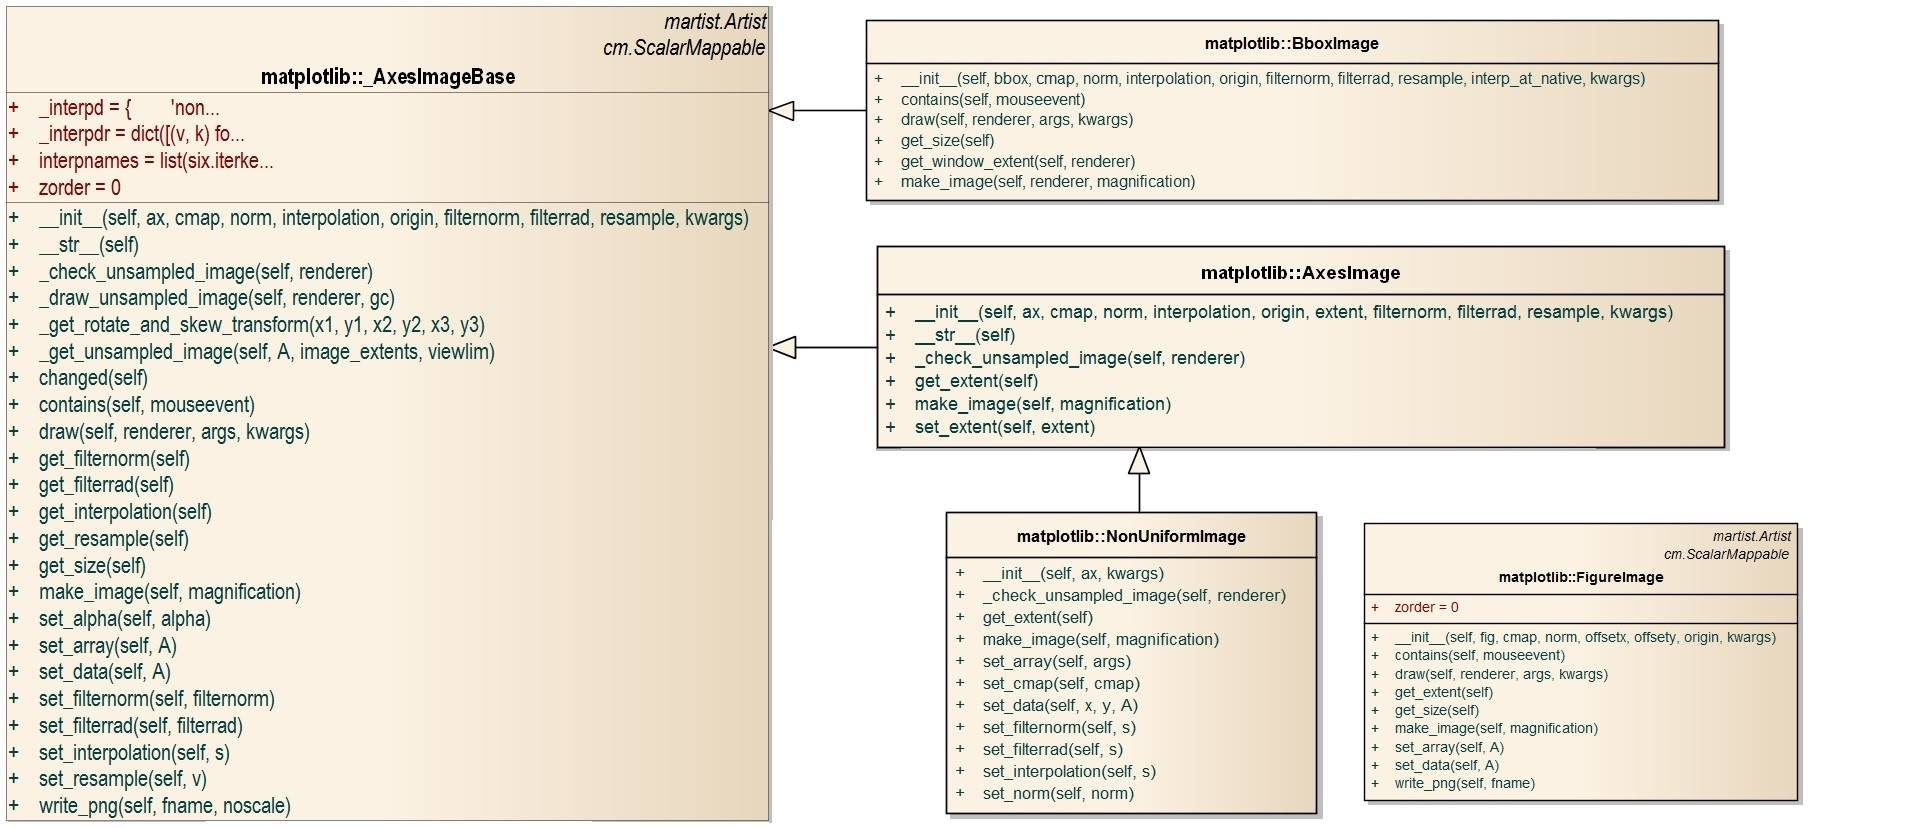
\includegraphics[width=0.8\textwidth]{img/umls/josh/img}
        \caption{The AxesImageBase class and its subclasses}\label{fig:math text}
\end{figure}


%S5--------------------------------------------------------------------------------------
\subsection{Mathtext}

Mathtext is a module for parsing a subset of the TeX math syntax and drawing them to a matplotlib backend. The base class for the mathtext backend-specific code.  The purpose of class: MathtextBackend subclasses is to interface between mathtext and a specific matplotlib graphics backend (see Figure~\ref{fig:math ext}).

\begin{figure}[ht!]
        \centering
                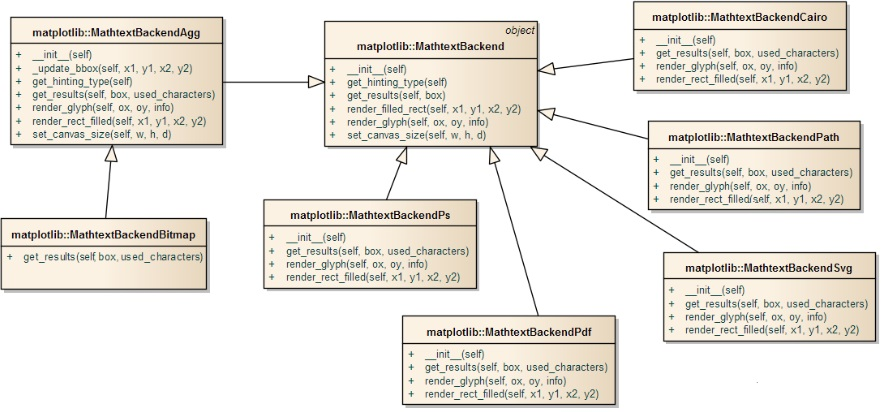
\includegraphics[width=0.5\textwidth]{img/umls/kevin/mathtext}
        \caption{The MathText class, which renders TeX math syntax}\label{fig:math text}
\end{figure}


\subsection{Colours \& CM}
Colors is a module for converting numbers or color arguments to *RGB* or *RGBA*, while cm (colormap) is a baseclass for all scalar to RGBA mappings (see Figure~\ref{fig:cm}).

\begin{figure}[ht!]
        \centering
                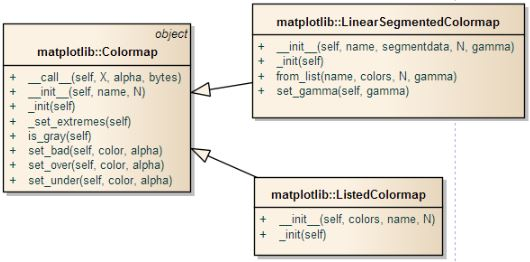
\includegraphics[width=0.5\textwidth]{img/umls/kevin/cm}
        \caption{The ColorMap class and its subclasses}\label{fig:cm}
\end{figure}

\begin{figure}[ht!]
        \centering
                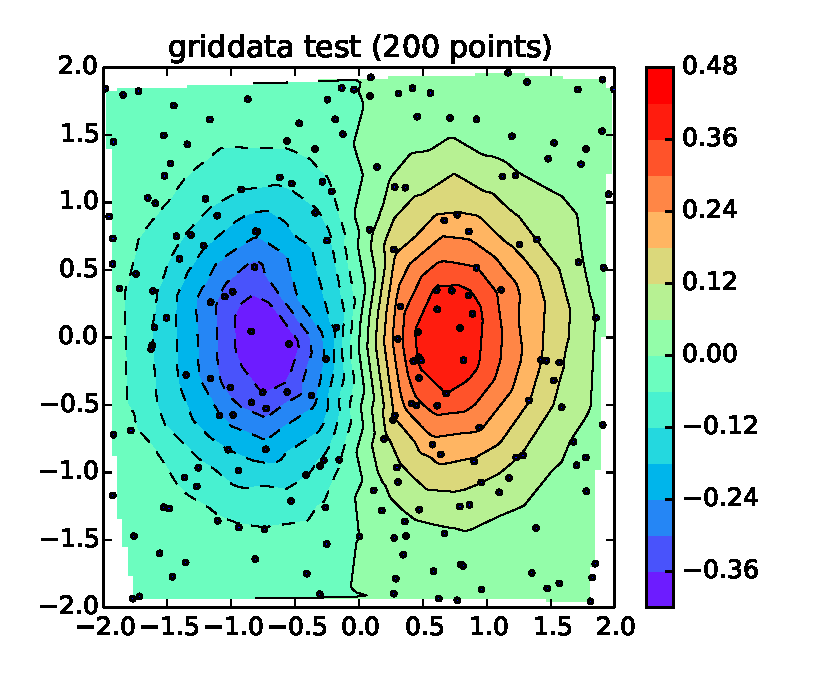
\includegraphics[width=0.3\textwidth]{img/umls/kevin/griddata}
        \caption{Example of colormap mapping data values to colours}\label{fig:artistExAgg}
\end{figure}

%S6--------------------------------------------------------------------------------------
\subsection{Annotation}

\begin{figure}[ht!]
        \centering
                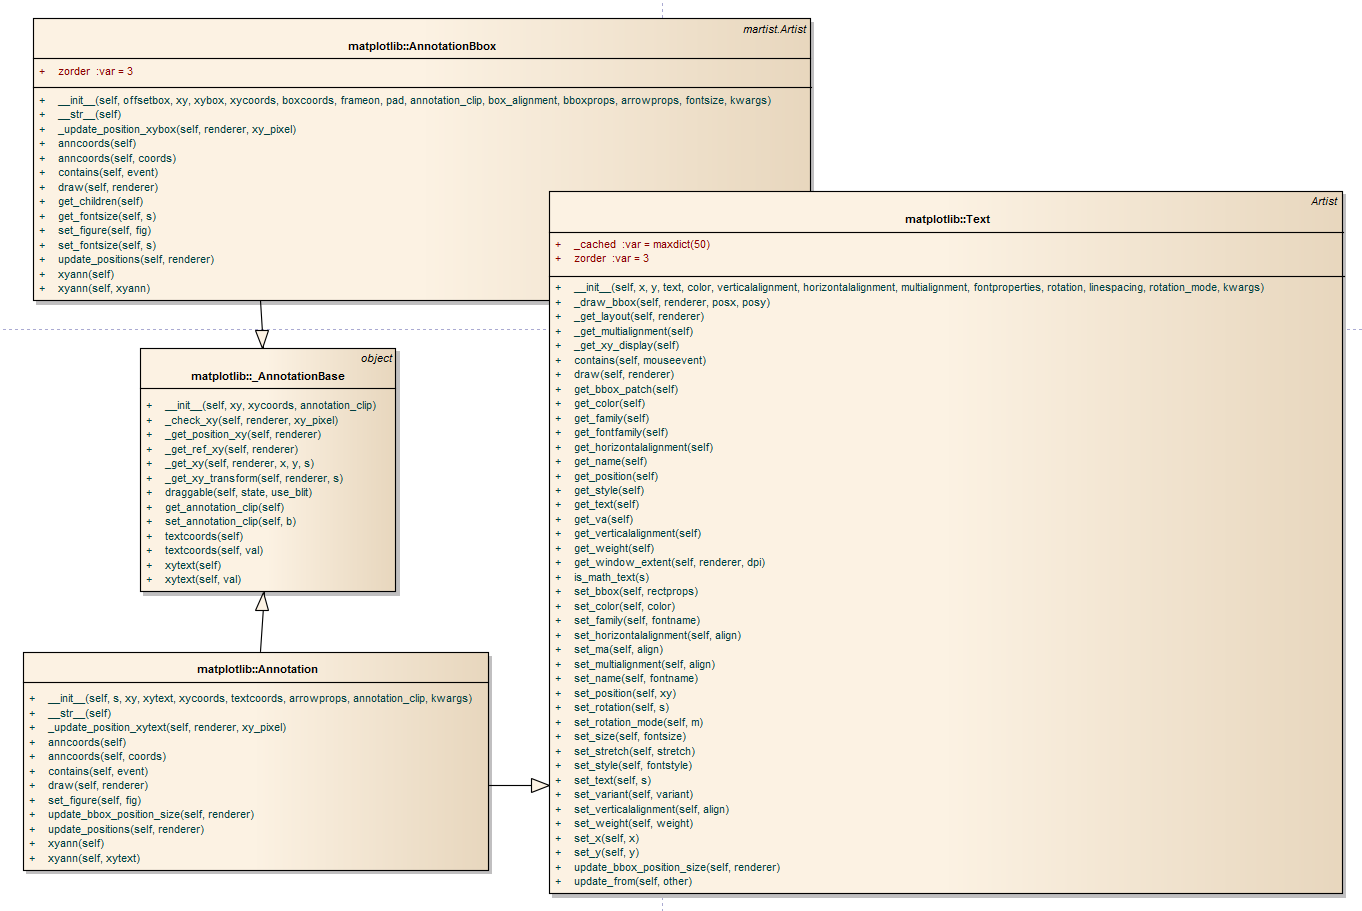
\includegraphics[width=0.4\textwidth]{img/umls/derek/annotation}
        \caption{The Text class and the Annotation classes}\label{fig:artistExAgg}
\end{figure}

\subsection{Patches}
Created by Composite Artists, Patches and its primitive artist subclasses creates patches of colour used as graphical elements that make up the plot background.
\begin{figure}[ht!]
        \centering
                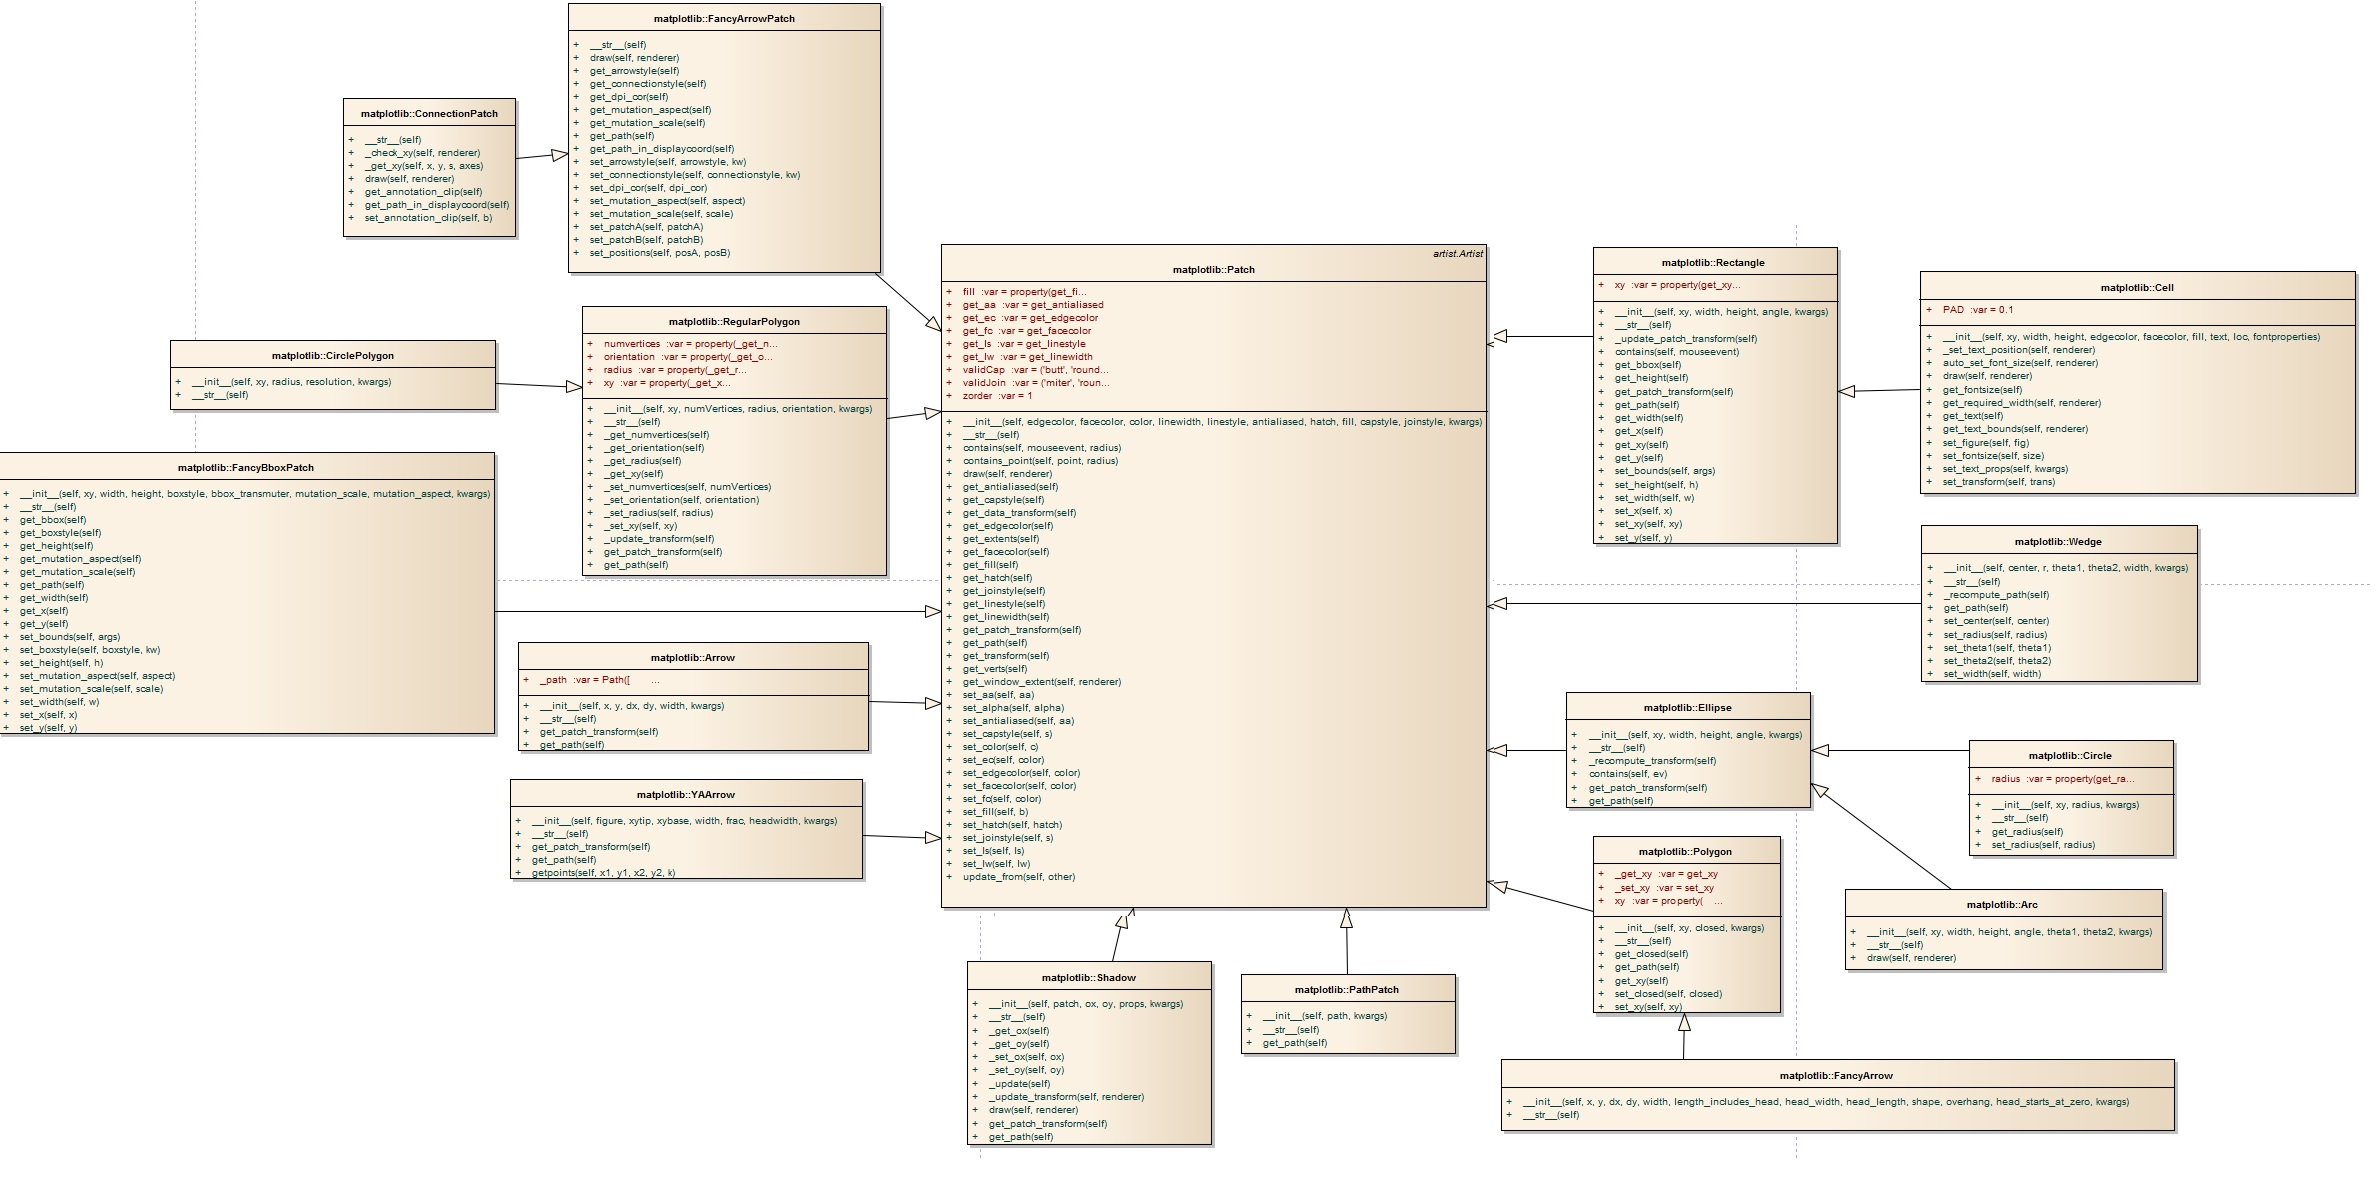
\includegraphics[width=\textwidth]{img/umls/derek/patch}
        \caption{The Patch class and many of its subclasses}\label{fig:artistExAgg}
\end{figure}

%S7--------------------------------------------------------------------------------------
\subsection{Artist}

The Artist class is an abstract class that is used to implement classes which is then used to display on the figureCanvas. These classes include Table, Line2D, Figure, Text, Legend etc?

\begin{figure}[ht!]
        \centering
                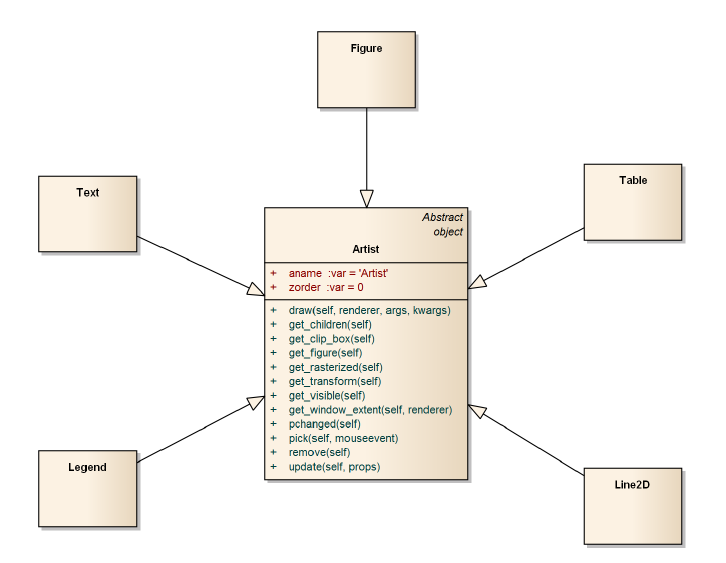
\includegraphics[width=0.5\textwidth]{img/umls/dave/artist}
        \caption{The Artist class and many of its subclasses}
\end{figure}

%S8--------------------------------------------------------------------------------------

\subsection{Style}

Style is a base class for all the styles. BoxStyle,  ConnectionStyle and ArrowStyle are subclasses of it. They are used to specify the location and size of the box to be drawn,  to create a path between two points, or to create an arrow path along a given path

\begin{figure}[ht!]
        \centering
                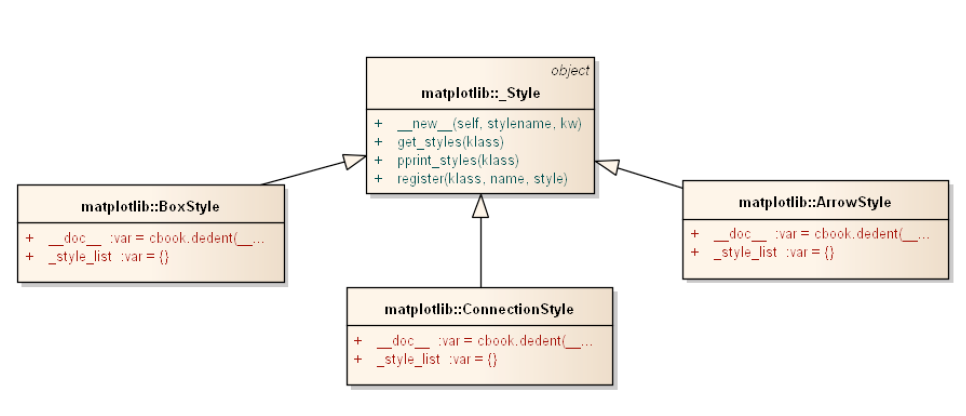
\includegraphics[width=0.5\textwidth]{img/umls/candy/style}
        \caption{The Style class and many of its subclasses}
\end{figure}

\subsection{ScaleBase}

ScaleBase: It is the base class for all scales. Scales are separable transformations, working on a single dimension. There are 3 different types of scale that can get transformed to. The default linear scale,  standard logarithmic scale and the symmetrical logarithmic scale

\begin{figure}[ht!]
        \centering
                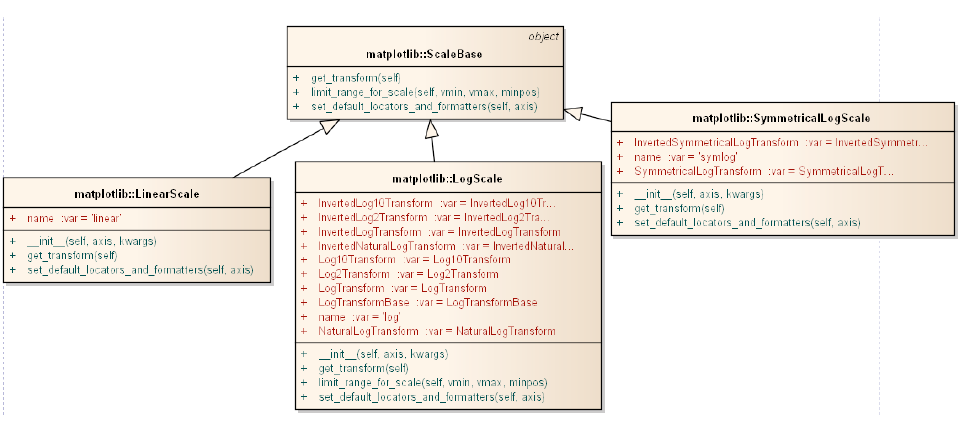
\includegraphics[width=0.5\textwidth]{img/umls/candy/Scale}
        \caption{The ScaleBase class and many of its subclasses}
\end{figure}

\subsection{RenderBase}

The Renderer Base is an abstract base class to handle drawing or rendering operations.


\begin{figure}[ht!]
        \centering
                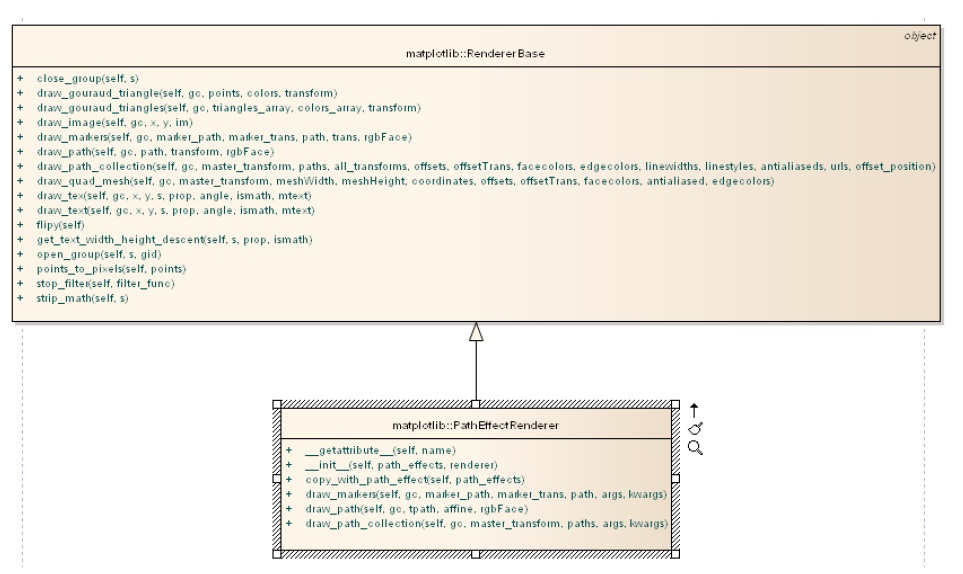
\includegraphics[width=0.5\textwidth]{img/umls/candy/Renderer}
        \caption{The Renderer class and many of its subclasses}
\end{figure}

\subsection{Path}

The class Path represents a series of possibly disconnected, possibly closed, line and curve segments. It has a subclass TextPath, which used to create a path from the text.


\begin{figure}[ht!]
        \centering
                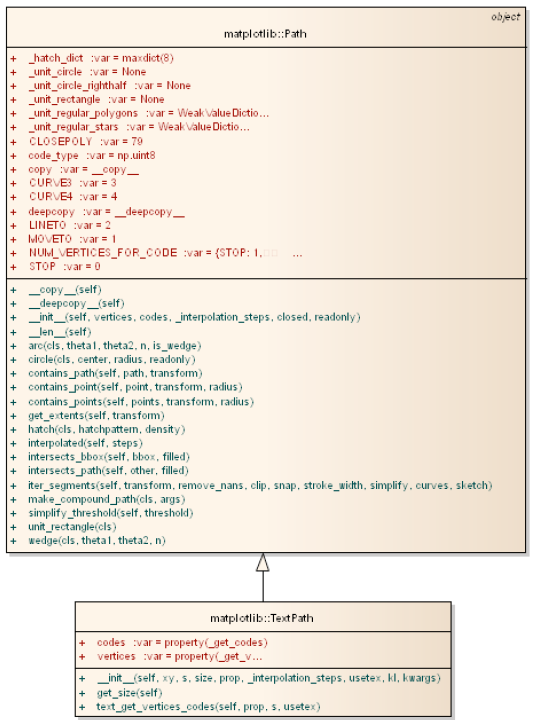
\includegraphics[width=0.5\textwidth]{img/umls/candy/Path}
        \caption{The Path class and many of its subclasses}
\end{figure}

\subsection{Widget}

The class Widget is an abstract base class for GUI neutral widgets. It contains widgets that are designed to work for any of the GUI backends. AxesWidget, SubplotTool and MultiCursor are the subclasses of the class Widget.

\begin{figure}[ht!]
        \centering
                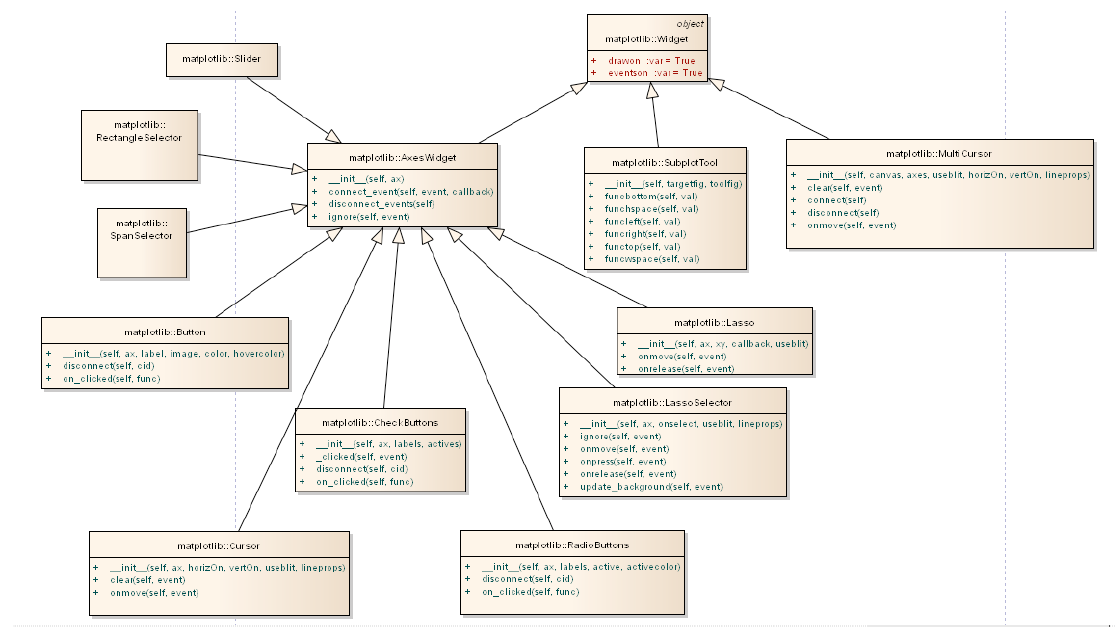
\includegraphics[width=0.5\textwidth]{img/umls/candy/Widget}
        \caption{The Artist class and many of its subclasses}
\end{figure}



%----------------------------------------------------------------------------------------
%xxxxxxxxxxxxxxxxxxxxxxxxxxxxxxxxxxxxxxxxxxxxxxxxxxxxxxxxxxx
%xxxxxxxxxxxxxxxxxxxxxxxxxxxxxxxxxxxxxxxxxxxxxxxxxxxxxxxxxxx

%\chapter{Chapter}
%\section{Section}
%\subsection{Subsection}
%\subsubsection{Subsubsection}
%\paragraph{Paragraph}

%\begin{figure}[ht!]
%\centering
%
\includegraphics[width=0.15\textwidth]{default}
%\caption[]{Default Img}
%\label{fig:overflow}
%\end{figure}

%xxxxxxxxxxxxxxxxxxxxxxxxxxxxxxxxxxxxxxxxxxxxxxxxxxxxxxxxxxx
%xxxxxxxxxxxxxxxxxxxxxxxxxxxxxxxxxxxxxxxxxxxxxxxxxxxxxxxxxxx
% END DOCUMENT
%xxxxxxxxxxxxxxxxxxxxxxxxxxxxxxxxxxxxxxxxxxxxxxxxxxxxxxxxxxx
%xxxxxxxxxxxxxxxxxxxxxxxxxxxxxxxxxxxxxxxxxxxxxxxxxxxxxxxxxxx

\end{document}